\documentclass[class=NCU_thesis, crop=false]{standalone}

\begin{document}

\chapter{研究方法}

\section{以卷積神經網路為基礎之新型可解釋性深度學習模型}
\subsection{模型架構}

此章節將介紹本論文所提出的可解釋性模型整體架構與每個部分的功能,並說明資料在模型中的運作方式,模型架構圖如\cref{fig:model_arch}。
整個模型可以分成三個部分,色彩感知區塊、輪廓感知區塊和特徵傳遞區塊。

\fig[1][fig:model_arch][H]{model_arch.png}[模型架構圖][模型架構圖]
\fig[1][fig:model_arch_simple][H]{model_arch_simple.png}[模型架構簡圖][模型架構簡圖]

這三種區塊均由不同的卷積模組、響應篩選模組、空間合併模組所組成。
卷積模組利用不同的方式學習與提取輸入的特徵,
響應篩選模組負責過濾不重要的特徵,
空間合併模組則模擬皮層的資訊合併,融合眼球跳動的概念,將輸入的資訊根據空間位置關係進行合併。

色彩感知區塊為單層架構,其架構如\cref{fig:color_arch}
透過彩色卷積模組計算輸入影像不同區塊的色彩與30種基本色彩的相似度去分析輸入影像的色彩分布,
並經過響應篩選模組、空間合併模組,以提取影像中每個區塊的色彩特徵。

\fig[0.5][fig:color_arch][H]{chapter3/color_arch.png}[色彩感知區塊架構圖][色彩感知區塊架構圖]

輪廓感知區塊也為單層架構,
透過將影像進行灰階前處理後,
使用高斯卷積模組、響應篩選模組、空間合併模組,
來提取影像中輪廓和邊緣的特徵。

\fig[0.5][fig:gray_arch][H]{chapter3/gray_arch.png}[輪廓感知區塊架構圖][輪廓感知區塊架構圖]

特徵傳遞區塊為多層架構,
使用了高斯卷積模組、特徵強化模組、空間合併模組
負責處理和學習前面感知區塊所提取的特徵。

\fig[0.5][fig:combine_arch][H]{chapter3/combine_arch.png}[特徵傳遞區塊架構圖][特徵傳遞區塊架構圖]

此外,為了在訓練之後使用者可以對彩色和灰階的可解釋性圖片進行對照,
因此我們對模型加入了一個限制,
限制色彩特徵傳遞區塊和輪廓特徵傳遞區塊的層數和空間合併方式必須相同並且
色彩感知區塊和輪廓感知區塊的高斯卷積模組 Filter 長寬必須相同。

\pagebreak

\subsection{模型符號說明}
	\begin{description}
		\item[]\textit{B}$_{in}$, \textit{H}$_{in}$, \textit{W}$_{in}$:輸入影像之長、寬

		\item[]\textit{FM}:卷積模組之濾波器
		\item[]\textit{RM}:輸入經過卷積模組和響應篩選模組所輸出的結果
		\item[]\textit{CI}:卷積模組之濾波器在資料集的對應影像
		\item[]\textit{SF}$_{i}$:第i層的空間合併模組的濾波器大小(Spatial Filter)
		\item[]\textit{H}$^{i}_{SF}$、\textit{W}$^{i}_{SF}$:第i層的空間合併模組輸出的長、寬

		\item[]\textit{FM}$^{color}_{0}$:色彩感知區塊之彩色卷積模組的\textit{FM}
		\item[]\textit{RM}$^{color}_{0}$:色彩感知區塊之彩色卷積模組的\textit{RM}
		\item[]\textit{CI}$^{color}_{0}$:色彩感知區塊之彩色卷積模組的\textit{FM}的對應影像
		\item[]\textit{H}$^{color}_{Filter}$, {W}$^{color}_{Filter}$: 色彩感知區塊之彩色卷積模組的濾波器長、寬
		\item[]\textit{C}$^{color}_{0}$, {H}$^{color}_{0}$, {W}$^{color}_{0}$:色彩感知區塊之輸出的通道數、長、寬

		\item[]\textit{FM}$^{color}_{i}$:色彩特徵傳遞區塊第i層之高斯卷積模組的\textit{FM}, i = 1$\sim$L
		\item[]\textit{RM}$^{color}_{i}$:色彩特徵傳遞區塊第i層之高斯卷積模組的\textit{RM}, i = 1$\sim$L
		\item[]\textit{CI}$^{color}_{i}$:色彩特徵傳遞區塊第i層之高斯卷積模組的\textit{FM}$_{i}$的對應影像, i = 1$\sim$L
		\item[]\textit{C}$^{color}_{i}$, \textit{H}$^{color}_{i}$, \textit{W}$^{color}_{i}$:色彩特徵傳遞區塊第i層之輸出的通道數、長、寬, i = 1$\sim$L
		
		\item[]\textit{FM}$^{gray}_{0}$:輪廓感知區塊之高斯卷積模組的\textit{FM}
		\item[]\textit{RM}$^{gray}_{0}$:輪廓感知區塊之高斯卷積模組的\textit{RM}
		\item[]\textit{CI}$^{gray}_{0}$:輪廓感知區塊之高斯卷積模組的\textit{FM}$^{gray}_{0}$的對應影像
		\item[]\textit{H}$^{gray}_{Filter}$, {W}$^{gray}_{Filter}$: 輪廓感知區塊之高斯卷積模組的濾波器長、寬
		\item[]\textit{C}$^{gray}_{0}$, \textit{H}$^{gray}_{0}$, {W}$^{gray}_{0}$:輪廓感知區塊之輸出的通道數、長、寬

		\item[]\textit{FM}$^{gray}_{i}$:輪廓特徵傳遞區塊第i層之高斯卷積模組的\textit{FM}, i = 1$\sim$L
		\item[]\textit{RM}$^{gray}_{i}$:輪廓特徵傳遞區塊第i層之高斯卷積模組的\textit{RM}, i = 1$\sim$L
		\item[]\textit{CI}$^{gray}_{i}$:輪廓特徵傳遞區塊第i層之高斯卷積模組的\textit{CI}$_{i}$的對應影像, i = 1$\sim$L
		\item[]\textit{C}$^{gray}_{i}$, \textit{H}$^{color}_{i}$, \textit{W}$^{color}_{i}$:輪廓特徵傳遞區塊第i層之輸出的通道數、長、寬, i = 1$\sim$L
	\end{description}

\subsection{演算法流程}
Step 1:決定整個模型的架構與參數,色彩特徵傳遞區塊與輪廓特徵傳遞區塊之層數均為L

Step 2:對輸入的彩色影像做灰階前處理產生對應的灰階影像

Step 3:將彩色影像(B$_{in}$, 3, H$_{in}$, W$_{in}$)和灰階影像(B$_{in}$, 1, H$_{in}$, W$_{in}$)分別輸入色彩提取層和輪廓提取層。各自的輸出為色彩輸出(B$_{in}$, 30, H$^{color}_{0}$, W$^{color}_{0}$),灰階輸出(B$_{in}$, C${_{gray}}$, H$^{gray}_{0}$, W$^{gray}_{0}$)

Step 4:將色彩輸出和灰階輸出分別輸入進各自的特徵傳遞層進行綜合特徵的學習與合併,
		最終會獲得色彩特徵(B$_{in}$, C$^{color}_{L}$, H$^{color}_{L}$, W$^{color}_{L}$), 灰階特徵(B$_{0}$, C$^{gray}_{L}$, H$^{gray}_{L}$, W$^{gray}_{L}$)

Step 5:將色彩特徵與灰階特徵攤平後concat成為(B$_{in}$, C$^{Linear}_{in}$)並輸入進全連接層學習分類特徵

Step 6:計算 loss value 並進行反向傳播


\pagebreak

\section{卷積模組設計與實現}
	% \subsection{卷積模組之實作優化}
	% 	在CIM的高斯卷積模組實作上,
	% 	採用了逐個計算每個 Windows 和濾波器之間的歐氏距離並將結果輸入進高斯函數得出相似度。
	% 	我們改進了這個實作過程,利用了 GPU 的多核優勢,
	% 	將每次卷積的所有位置的 Windows 取出來後平行放入 GPU 的多個核心,
	% 	同時計算這些 Windows 與濾波器的歐氏距離再輸入高斯函數中得出相似度,
	% 	並將這個平行處理方式應用在所有的卷積模組中。
	% 	這樣的實作方式使得整體模型的訓練速度可以大幅提高,
	% 	也完整利用GPU的效能,提升了模型效率。

	\subsection{彩色卷積模組的設計與實現}
		彩色卷積模組為色彩感知區塊的卷積模組,
		該模組主要是透過將濾波器(Filter)設定30個調色基礎顏色的色塊來作為該區塊的權重,
		並使用彩色卷積模組計算出影像中不同區塊之色彩與Filter色彩的響應值。
		以下將針對濾波器之設計、彩色卷積模組,兩個部分進行詳細說明。
		
		\subsubsection{濾波器之設計}
			由於色彩提取區塊的輸入為彩色影像其輸入通道分別為紅、綠、 藍三色的通道,
			我們設定輸出的通道數為固定為30,
			使得濾波器的形狀為 $\left(30 , 3, H^{color}_{Filter},  W^{color}_{Filter} \right)$,
			並將其為 30 種不同RGB色彩的$H^{color}_{Filter} * W^{color}_{Filter}$色塊。

			在30種不同色彩的選擇上,
			我們採用日本色彩研究所於1965年提出的PCCS(Practical Color Co-ordinate System)中的24色相環中(如\cref{fig:PCCS}所示)的顏色,
			再加上紅、綠、藍、黑、白、灰六個基礎色組成。
			由於以上的30色均為基礎顏色(如\cref{fig:30Base}),
			因此我們希望透過計算不同區塊的色彩與這些基礎顏色的響應值來當作區塊的色彩特徵。

			\fig[0.4][fig:PCCS][H]{chapter3/PCCS.jpg}[PCCS體系的24色色相環\cite{PCCScite}][PCCS體系的24色色相環]

			\fig[0.4][fig:30Base][H]{chapter3/30BaseColor.png}[濾波器設定的基礎30色][濾波器設定的基礎30色]

		\subsubsection{彩色卷積模組}
			\label{chapter:color_convolution}
			在傳統的卷積操作中,
			我們會在輸入影像上使用一個稱為Slide Windows的滑動窗口,
			並且與不同的濾波器進行內積運算來計算輸出,
			這樣的輸出結果只能代表Windows與不同濾波器在平面上的投影而並沒有相似度的意義。
			然而我們在彩色感知區塊的濾波器視為不同的色彩,
			因此我們在計算Windows時會將透過將Windows內的所有像素的RGB值進行加總與平均,
			計算出該Windows的平均RGB值作為該Windows的代表色。
			之後我們計算Windows的代表色與濾波器中不同的顏色的色差,
			並且利用高斯函數取代內積運算將色差轉換為相似度,
			以相似度作為反應強度進行輸出。

			\fig[0.5][fig:colorConvolution][H]{chapter3/color_convolution.png}[彩色卷積示意圖][彩色卷積示意圖]

			在色差的計算上,我們使用由CompuPhase公司提出的一種低成本的加權歐氏距離公式\cite{LABformula}(簡稱LAB Euclidean),
		  	它的權重由RGB中的紅色在色彩中的分量多少而決定。
		  	這種色差計算方法的好處是利用這個公式便可以用兩個顏色的RGB值計算出接近CIE L*a*b(CIE L*u*v)空間中的距離,
		  	同時這套公式也被使用在CompuPhase自己的產品中。
		  	CIE L*a*b是由國際照明委員會提出的色彩空間,
		  	是目前描述人眼可見所有顏色最完整的色彩空間,
		  	因此在CIELAB的距離也會較RGB空間之距離更接近人眼所視。
		  	其公式如\cref{eq:eq-LAB},
		  	其中C$_{1}$代表第一個顏色,
		  	C$_{2}$代表第二個顏色。
		  	\begin{equation}
		    \label{eq:eq-LAB}
		    \begin{split}
		    	\overline{r} & = \frac{C_{1,R} + C_{2,R}}{2} \\
		    	\Delta R & = C_{1,R} - C_{2,R} \\
		    	\Delta G & = C_{1,G} - C_{2,G} \\
		    	\Delta B & = C_{1,B} - C_{2,B} \\
		    	\Delta C & = \sqrt{(2 + \frac{\overline{r}}{256}) * (\Delta R)^2 + 4 * (\Delta G)^2 + (2 + \frac{255 - \overline{r}}{256}) * (\Delta B)^2}
		    \end{split}
			\end{equation}

			\fig[0.5][fig:LabColorSpace][H]{chapter3/Lab_color_space.jpg}[CIE L*a*b 色彩模型][CIE L*a*b 色彩模型]

			% 在色差的計算上,我們曾經考慮過下面三種不同的色差計算方法,分別如下:
			% \begin{itemize}
			%   \item [1)] 
			%   	計算RGB色彩空間的歐氏距離(Euclidean Distance)來代表顏色之間的差距,
			%   	其公式如\cref{eq:eq-RGBcdist}。
			%   	他是三種方法之中最為快速
			%   	$\Delta$C代表兩個顏色的色差,
			%   	$\Delta$R為兩個顏色R值的差距,
			%   	$\Delta$G為兩個顏色G值的差距,
			%   	$\Delta$B為兩個顏色B值的差距。
			%   	\begin{equation}
			%     \label{eq:eq-RGBcdist}
			%     	\Delta C = \sqrt{(\Delta R)^2 + (\Delta G)^2 + (\Delta B)^2}
			% 	\end{equation}

			%   \item [2)]
			%   	由CompuPhase公司提出的一種低成本的加權歐氏距離公式\cite{LABformula}(簡稱LAB Euclidean),
			%   	它的權重由RGB中的紅色在色彩中的分量多少而決定。
			%   	這種色差計算方法的好處是利用這個公式便可以用兩個顏色的RGB值計算出接近CIE L*a*b(CIE L*u*v)空間中的距離,
			%   	同時這套公式也被使用在CompuPhase自己的產品中。
			%   	CIE L*a*b是由國際照明委員會提出的色彩空間,
			%   	是目前描述人眼可見所有顏色最完整的色彩空間,
			%   	因此在CIELAB的距離也會較RGB空間之距離更接近人眼所視。
			%   	其公式如\cref{eq:eq-LAB},
			%   	其中C$_{1}$代表第一個顏色,
			%   	C$_{2}$代表第二個顏色。
			%   	\begin{equation}
			%     \label{eq:eq-LAB}
			%     \begin{split}
			%     	\overline{r} & = \frac{C_{1,R} + C_{2,R}}{2} \\
			%     	\Delta R & = C_{1,R} - C_{2,R} \\
			%     	\Delta G & = C_{1,G} - C_{2,G} \\
			%     	\Delta B & = C_{1,B} - C_{2,B} \\
			%     	\Delta C & = \sqrt{(2 + \frac{\overline{r}}{256}) * (\Delta R)^2 + 4 * (\Delta G)^2 + (2 + \frac{255 - \overline{r}}{256}) * (\Delta B)^2}
			%     \end{split}
			% 	\end{equation}

			% 	\fig[0.5][fig:LabColorSpace][H]{chapter3/Lab_color_space.jpg}[CIE L*a*b 色彩模型][CIE L*a*b 色彩模型]
				

			%   \item [3)]
			%   	根據2019年提出的伽馬校正論文\cite{GammaCorrection}中所述,
			%   	人們對於每個顏色的亮度感知呈現不同的非線性曲線,
			%   	因此對於不同的色彩的權重應該要是不同的。
			%   	我們參考了\cite{LABformula}提及的加權歐氏距離的公式(之後簡稱Weighted Euclidean),
			%   	公式如\cref{eq:eq-weightcdist}。
			%   	\begin{equation}
			%     \label{eq:eq-weightcdist}
			%     	\Delta C = \sqrt{2 * (\Delta R)^2 + 4 * (\Delta G)^2 + 3 * (\Delta B)^2}
			% 	\end{equation}
			% 	然而,在\cite{LABformula}中也有提到,根據伽馬校正的理論,或許我們應該對不同的顏色分布的影像設定不同的加權值才會比較符合人眼的視覺對顏色亮度的感知。
			% \end{itemize}
			% 這三個色差的計算方法各有其優缺點,
			% 並且經過我們的實驗(實驗詳細於\cref{chapter:diff-colordist-compare})後發現三者在準確度和可解釋圖片的產生上十分相似,
			% 但考量到Euclidean方法會容易受到RGB值的細微不同而產生變化。
			% 而根據上面提到\cite{LABformula}中的說法,
			% 如果使用Weight Euclidean方法會需要因應不同的資料集去調整加權數值,會增加問題的複雜度。
			% 因此我們最終選擇了穩定性較高的LAB Euclidean方法來計算色彩感知區塊中輸入影像和30類基礎顏色的色差值,
			% 之後將色差值輸入高斯函數中做為評估相似度的依據。

	\subsection{灰階前處理的設計與實現}
		在輪廓感知區塊中,
		為了使該區塊能夠專注於提取輪廓特徵而不需考慮色彩因素,
		我們會對輸入影像進行前處理。
		首先,我們會將彩色影像轉換為灰階影像,
		轉換公式如\cref{eq:eq-grayscale},
		Gray代表灰階值,R、G、B各代表紅、綠、藍三色通道的值。
		\begin{equation}
		    \label{eq:eq-grayscale}
		    Gray = 0.299 * R + 0.587 * G + 0.114 * B
		\end{equation}
		這種加權方法主要考慮了人眼對於不同色彩的敏感度,
		從而能夠較為完整保留彩色圖像中的細節,
		接著為了消除不同色彩導致的灰度值差異,
		使該區塊能夠專注於輪廓資訊而不考慮色彩資訊,
		我們接者進行了Min-max正規化,
		使每張影像的灰階值統一至[$0, 1$]之間。
		透過上面步驟的前處理,
		我們從而可以確保輪廓感知區塊能夠專注於提取輪廓的特徵。

		\fig[0.7][fig:grayscale][H]{chapter3/grayscale.png}[灰階前處理示意圖][灰階前處理示意圖]

	\subsection{高斯卷積模組的設計與實現}
		\subsubsection{濾波器初始化}
			在這個模型之中,除了色彩感知區塊外,
			其餘區塊的高斯卷積模組的濾波器我們均是使用 Kaiming Uniform \cite{DBLP:journals/corr/HeZR015}的方式初始化濾波器的參數。
			初始化範圍為$[-\sqrt{\frac{6}{\text{fan\_in}}}, \sqrt{\frac{6}{\text{fan\_in}}}]$,
			$\text{fan\_in}$ 為輸入通道數。

			我們在實作中選擇使用 Kaiming Uniform 的原因是因為 Kaiming Uniform 相較於常用的 Uniform 初始化和 Xavier Uniform\cite{pmlr-v9-glorot10a} 初始化多考慮了整流線性單位函數(ReLU)等非線性激活函數的存在,
			Uniform 初始化的方式無法解決隨著神經網路的增加而導致梯度消失的問題,
			Xavier Uniform 為了解決梯度消失問題加入了 rescale 函數 $\frac{1}{\sqrt{\text{n}}}$但卻只適用於激活函數為線性函數的情況下,
			而 Kaiming Uniform 在解決梯度消失的問題時同時考慮了激活函數為非線性函數的情況並在\cite{DBLP:journals/corr/HeZR015}透過實驗證明了kaiming uniform 在神經網路在不影響準確度的同時更快收斂。
			由於我們的模型中在響應篩選模組中使用的非線性函數ReLU的變形去進行響應篩選,因此選擇了 Kaiming Uniform 來去進行後面的實驗。

		\subsubsection{高斯卷積模組}
			在高斯卷積模組中,
			流程如下,
			首先分別計算每個濾波器與卷積中的每個Slide Windows的歐氏距離
			其公式如\cref{eq:eq-EulideanDist},
			Windows$_{i}$ 為 Window 中第i個pixel值, 
			Filter$_{i}$為濾波器中第i個pixel值,
			C$_{in}$為輸入的channel數,
			Filter$_{H}$, Filter$_{W}$ 為卷積的濾波器大小,
			dist為該濾波器與Window的歐氏距離。
			在得到每個濾波器與每個Windows之間的歐氏距離後,
			再將其輸入高斯函數計算出每個濾波器每個Windows之間的相似度,
			並將其作為響應值進行輸出。

			\begin{equation}
			    \label{eq:eq-EulideanDist}
			    dist = \sqrt{\sum_{i = 1}^{K} (Windows_{i} - Filter_{i})^{2}} \quad where \; K = Filter_{H} * Filter_{W} * C_{in}
			\end{equation}

				我們在此利用高斯函數取代內積的原因在於高斯函數是以距離為基礎的函數,
			其計算結果能夠反映出距離的意義並且表達向量間的相似度,
			而相似度在後續的解釋性表現中幫助我們更好的理解模型的可解釋性圖片產生之原因。\\
			高斯函數(Gaussian function):\\
			  $x$ 為輸入值、$m$ 為中心點、$\sigma$ 為寬度參數
			  \begin{equation}
			      \label{eqn:rbf-gaussian-function}
			      \phi (x) = \exp \left( -\frac{dist^2}{2\sigma ^2} \right) 
			  \end{equation}

		  	此外,我們在選擇如何將距離轉換成相似度的函數時,
		  	也嘗試了\cite{YangCNNInterpretable}中提到了一個三角形的放射狀基底函數(以下簡稱Triangle函數)
		  	其公式如\cref{eqn:rbf-triangle-function},x為輸入值,m為中心點,w為寬度參數。
		  	\begin{equation}
		      \label{eqn:rbf-triangle-function}
		      \phi (x) = 1 - \frac{ \max \left( dist, w \right)}{w}
		  	\end{equation}

		  	\begin{figure}[H]
		    \centering
		    \subcaptionbox
		        {高斯函數
		        \label{fig:gaussian}}
		        {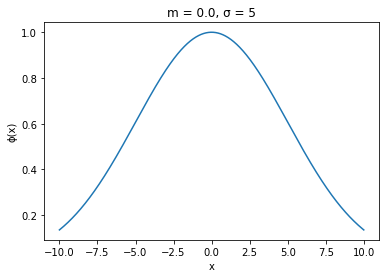
\includegraphics[width=0.33\linewidth]{chapter3/gaussian.png}}
		    ~
		    \subcaptionbox
		        {Triangle函數
		        \label{fig:triangle}}
		        {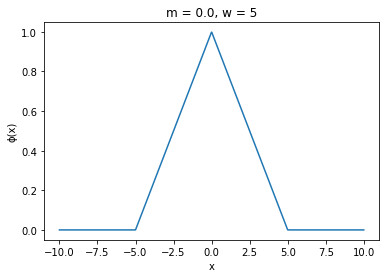
\includegraphics[width=0.33\linewidth]{chapter3/triangle.png}}
		    \caption{高斯函數與Triangle函數\cite{YangCNNInterpretable}}
		    \label{fig:rbf}
			\end{figure}

\section{FM、 RM的定義}
	特徵映射圖(FM)為將卷積模組的濾波器提取出來的結果,
	由於模型在高斯卷積模組為計算輸入濾波器與相似度,
	因此FM可以被視為模型學習到了輸入影像中的何種特徵。

	\fig[0.5][fig:FM_picture][H]{chapter3/FM.png}[FM示意圖][FM示意圖]

	特徵映射響應圖(RM)為當輸入進入卷積模組後所得到的輸出,
	其代表的是輸入區域對於該高斯卷積模組的濾波器的相似度,
	也被視為輸入對該高斯卷機模組所有的濾波器的反應強度。
	同一層、不同位置的RM數值為輸入影像的不同位置對於某個濾波器的反應,
	不同層、同一位置的RM數值為輸入影像的同一位置對於不同濾波器的反應。

	\fig[0.7][fig:RM_picture][H]{chapter3/RM-example.png}[RM示意圖][RM示意圖]

\pagebreak

\section{響應篩選模組之設計}
	% 在響應篩選模組中,
	% CIM 使用了自行設計的增強特徵的整流線性單位函數(changed ReLU, 簡稱cReLU),
	% 希望透過閥值過濾不重要的特徵,其公式如\cref{eq:eq-crelu}所示,
	
	% 作為閥值的 $c$ 值需要透過觀察資料集在高斯卷積模組的輸出來設定具體不同的$c$的數值來適應不同的資料集。
	% 然而一旦閥值設定過小則會削弱響應篩選的效果,
	% 閥值設定過大則會將大部分的特徵都歸零導致無法學習出有效特徵,
	% 因此如何設定 $c$ 則成為一個非常困難的問題,並且每次更換資料集都必須面對這個問題。

	% 為了解決閥值設定的問題,
	% 我們對cReLU的公式進行改善,
	
	響應篩選模組的主要目的是過濾卷積後響應較弱的值,
	保留響應較強的值,
	從而在後續產生可解釋性圖片時能有更好的呈現效果。

	我們將輸入的所有RM的響應值總個數$N_{RM}$,
	並設定一個希望保留的RM的百分比參數 $p\%$,
	這代表我們希望保留所有RM中響應值最大的前$p\%$的元素。
	接著從RM中取出第 $p\% * N_{RM}$  個最大的元素稱之為$P_{RM}$,
	並且將所有小於$P_{RM}$的數值歸零,
	篩選公式如\cref{eq:eq-cReLUPercent}。
	此公式代表的意義為保留響應值前$p\%$最大的值並刪除其餘響應值較弱的值。
	
	篩選公式為\\
	\begin{equation}
	    \label{eq:eq-cReLUPercent}
	    f(x)= 
	    \begin{cases}
	        0 & \text{if  $x < P_{RM}$ }\\
	        x & \text{if  $x \geq P_{RM}$}
	    \end{cases} \quad where \; P_{RM} = RM\left[ p\% * N_{RM} \right]
	\end{equation}
\pagebreak

\section{空間合併模組之設計}
	% 在空間合併模組上,
	% CIM為了保留 $RM$ 之間的空間位置關係簡化了眼球跳動的方式,
	% 加入了一個可訓練的時間遺忘函數 $\alpha$ 進入合併公式,其公式如\cref{eq:eq-sf}。
		
	% 這樣會導致越早被看到(時間越早)的數值需要乘上的 $\alpha^{k}$ 的 $k$ 值越大,
	% 在合併時的加權也就越小。
	% 儘管這種做法確實可以使輸出值呈現出空間上的關係,
	% 然而當我們需要合併的$RM_{k}$越多時,
	% 隨著$k$ 值越來越大,$\alpha^{k}$會快速變小。
	% 這樣便造成當我們將數值乘上過小的的$\alpha^{k}$後,
	% 便會變得這個數值便會在最終合併結果中變得無足輕重。
	% 對於大小較大的影像而言這種方法是有問題的,
	% 這會使得影像逐漸喪失一部分特徵。

	% 此外,
	% 在 CIM 的空間合併模組中為了方便輸出可視化圖片
	% 在實作上對輸入進行了維度轉換,
	% 將最後一維 Reshape 成一個二維矩陣,
	% 稱為特徵響應圖(RM)(其操作如\cref{fig:RM_picture}),
	% 然後乘上$\alpha$值進行合併。
	% 然而,我們認為此步驟會造成兩個問題:
	% 首先,CIM原本在第一層高斯卷積後的高斯卷積模組都只是做(1,1)的卷積操作,
	% 但是加入了這個步驟就會導致後續的高斯卷積模組的濾波器大小改變,容易引起閱讀者的誤解;
	% 其次,這個步驟並不會增加準確度或是增加效能,反而是多一些所轉置與Reshape所需要的時間。
	% 基於以上原因我們決定將此步驟捨棄。
	% 在空間合併模組前不再進行維度轉換和Reshape,
	% 並將輸入重新命名為GFR(Gaussian Feature Response),
	% 以區別於原來的RM。
	% 由於我們在空間合併模組前並沒有進行維度轉換和Reshape,
	% 因此公式的輸入使用RM的代稱已不再準確,
	% 所以我們將沒有進行轉換的空間合併模組輸入重新命名為GFR(Gaussian Feature Response)
	% 來與原來的RM做區分。

	在空間合併模組中,
	我們模擬皮層的層狀合併架構(\cref{fig:CorticalHierarchy})和眼球跳動的概念(\cref{fig:Saccade}),
	運用不同的加權參數值模擬眼球跳動的順序,
	將RM根據其空間位置關係對應到不同的加權參數值後進行合併,
	使得下一層卷積模組能夠在考慮特徵空間位置的前提下學習更大範圍的特徵。

	其步驟如下:
	一組輸入資訊經過卷積模組和響應篩選模組後會產生一個RM三維矩陣,
	一張輸入影像為多組輸入資訊的集合,因此產生多個RM矩陣,
	並且將這些RM根據 $SF_{i}$ 透過\cref{eq:eq-sf-update}進行合併,
	產生新的累積特徵響應圖(ARM)並輸入到下一層。

	為了保留RM之間的空間關係,
	我們先從[ $0.9 \sim 0.99$ ]之間進行等距採樣由小到大得到 $k$ 個值,
	將其稱為$\beta_{k}$。
	k 越小代表越早被眼球注視,k越大表示越晚被眼球注視,
	並按照RM合併的順序,
	將RM和$\beta_{k}$相乘並加總。
	其合併公式如\cref{eq:eq-sf-update},
	$ARM_{c}$為合併後的ARM,
	$RM_{k}$為第k個RM,
	$\beta_{k}$為從[$0.9 \sim 0.99$]之間取出的第$k$個值,
	${H}_{i}^{SF}$、${W}_{i}^{SF}$為第i層空間合併模組輸出的長和寬:\\
		\begin{equation}
		    \label{eq:eq-sf-update}
		    ARM_{c}=\frac{1}{n} \sum_{k = 0}^{n-1} \beta_{k} \times RM_{k}  \quad where \; n = \textit{H}^{i}_{SF} \times \textit{W}^{i}_{SF}
		\end{equation}

	% 得到 $k$ 個值代替 $\alpha^{k}$ 按照時序順序去乘以GBF ,
	% 我們將第 $k$ 個 $GFR$ 所對應的 $\alpha$ 稱為 $\beta_{k}$,
	% 如此便可以改善當需要合併的 $RM$ 數量過多時 $\alpha^{k}$ 過小的問題,
	% 同時也保留了CIM當初設計時希望保留的輸入之間的對應空間關係。\\
	
	
	RM的優化後的合併示意圖如\cref{fig:SFN_update}。
	\fig[0.5][fig:SFN_update][H]{chapter3/SFM_update.png}[優化後空間位置保留機制示意圖][優化後空間位置保留機制]


\pagebreak
\section{可解釋性} 
本研究以RM-CI做為解析模型的決策過程的基礎,
使得模型的決策過程可以被視覺化出來,
讓使用者了解模型關注的特徵資訊與決策背後的邏輯關係。

	\subsection{CI的意義}
	\label{section:InterablePicture}
	% \begin{figure}[H]
    % \centering
    % \subcaptionbox
    %     {$FM^{color}_0$
    %     \label{fig:FM_color_0}}
    %     {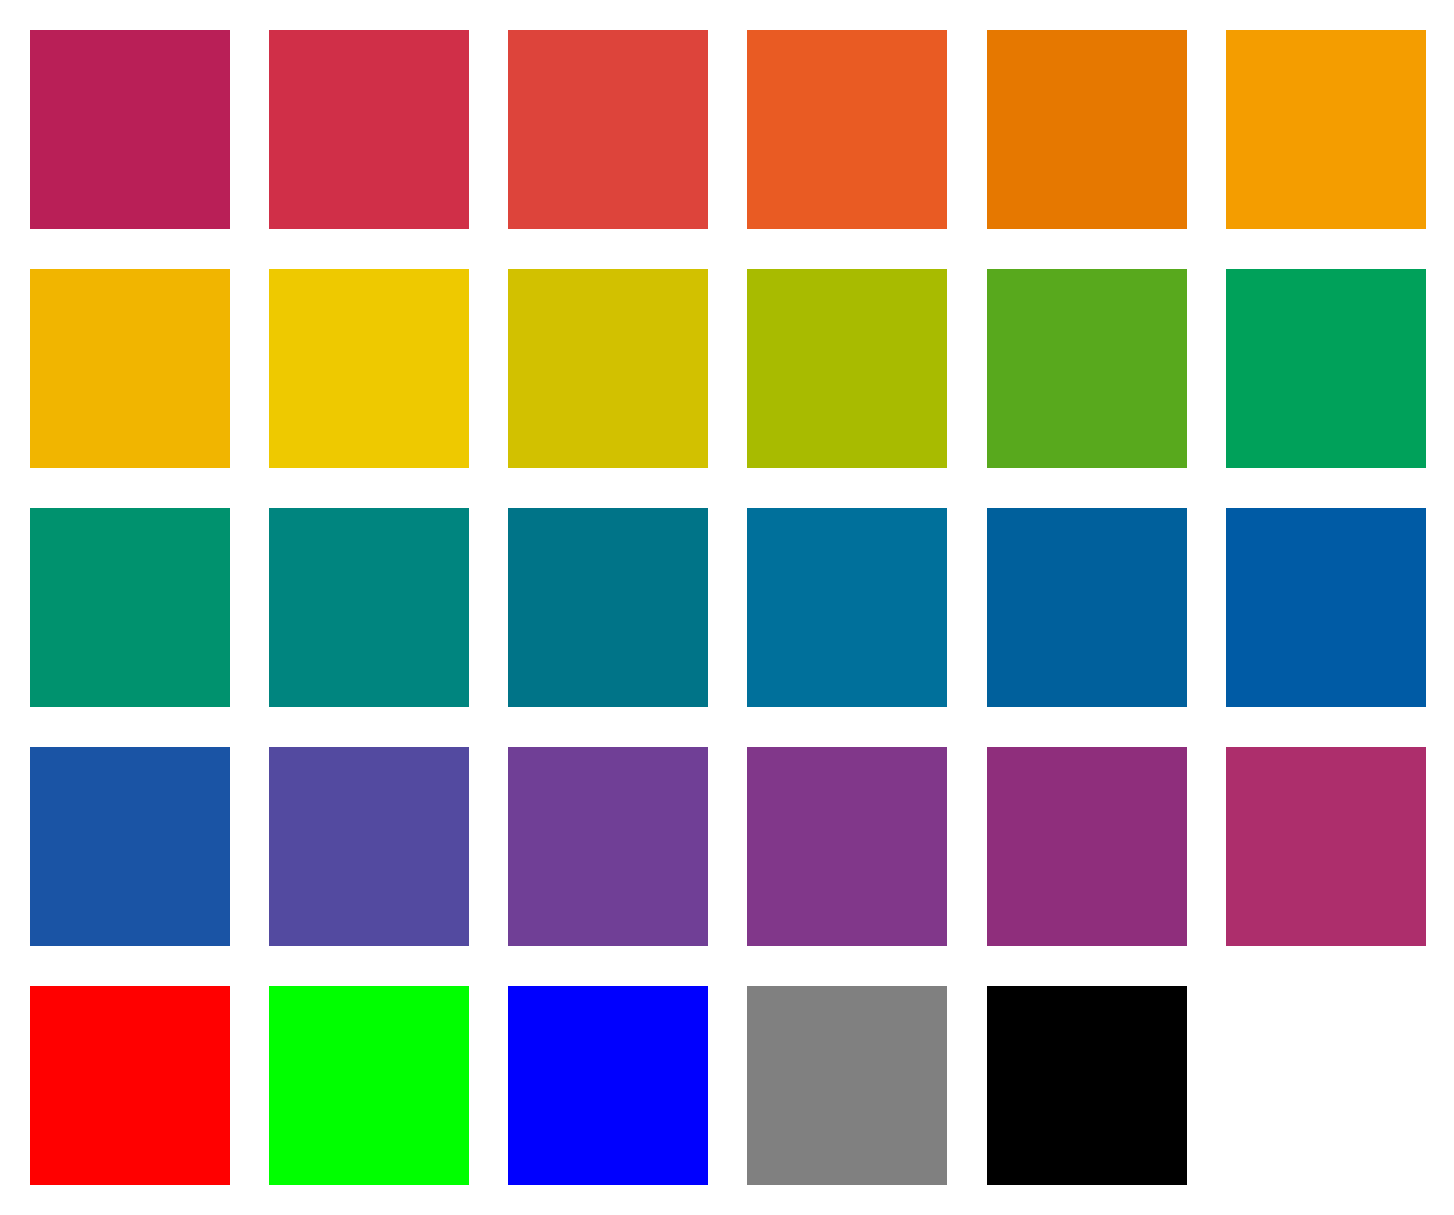
\includegraphics[width=0.3\linewidth]{chapter3/FMs/FMs_RGB_convs_0.png}}
    % ~
    % \subcaptionbox
    %     {$FM^{color}_1$
    %     \label{fig:FM_color_1}}
    %     {\includegraphics[width=0.3\linewidth]{chapter3/FMs/FMs_RGB_convs_1.png}}
    % ~
    % \subcaptionbox
    %     {$FM^{color}_2$
    %     \label{fig:FM_color_2}}
    %     {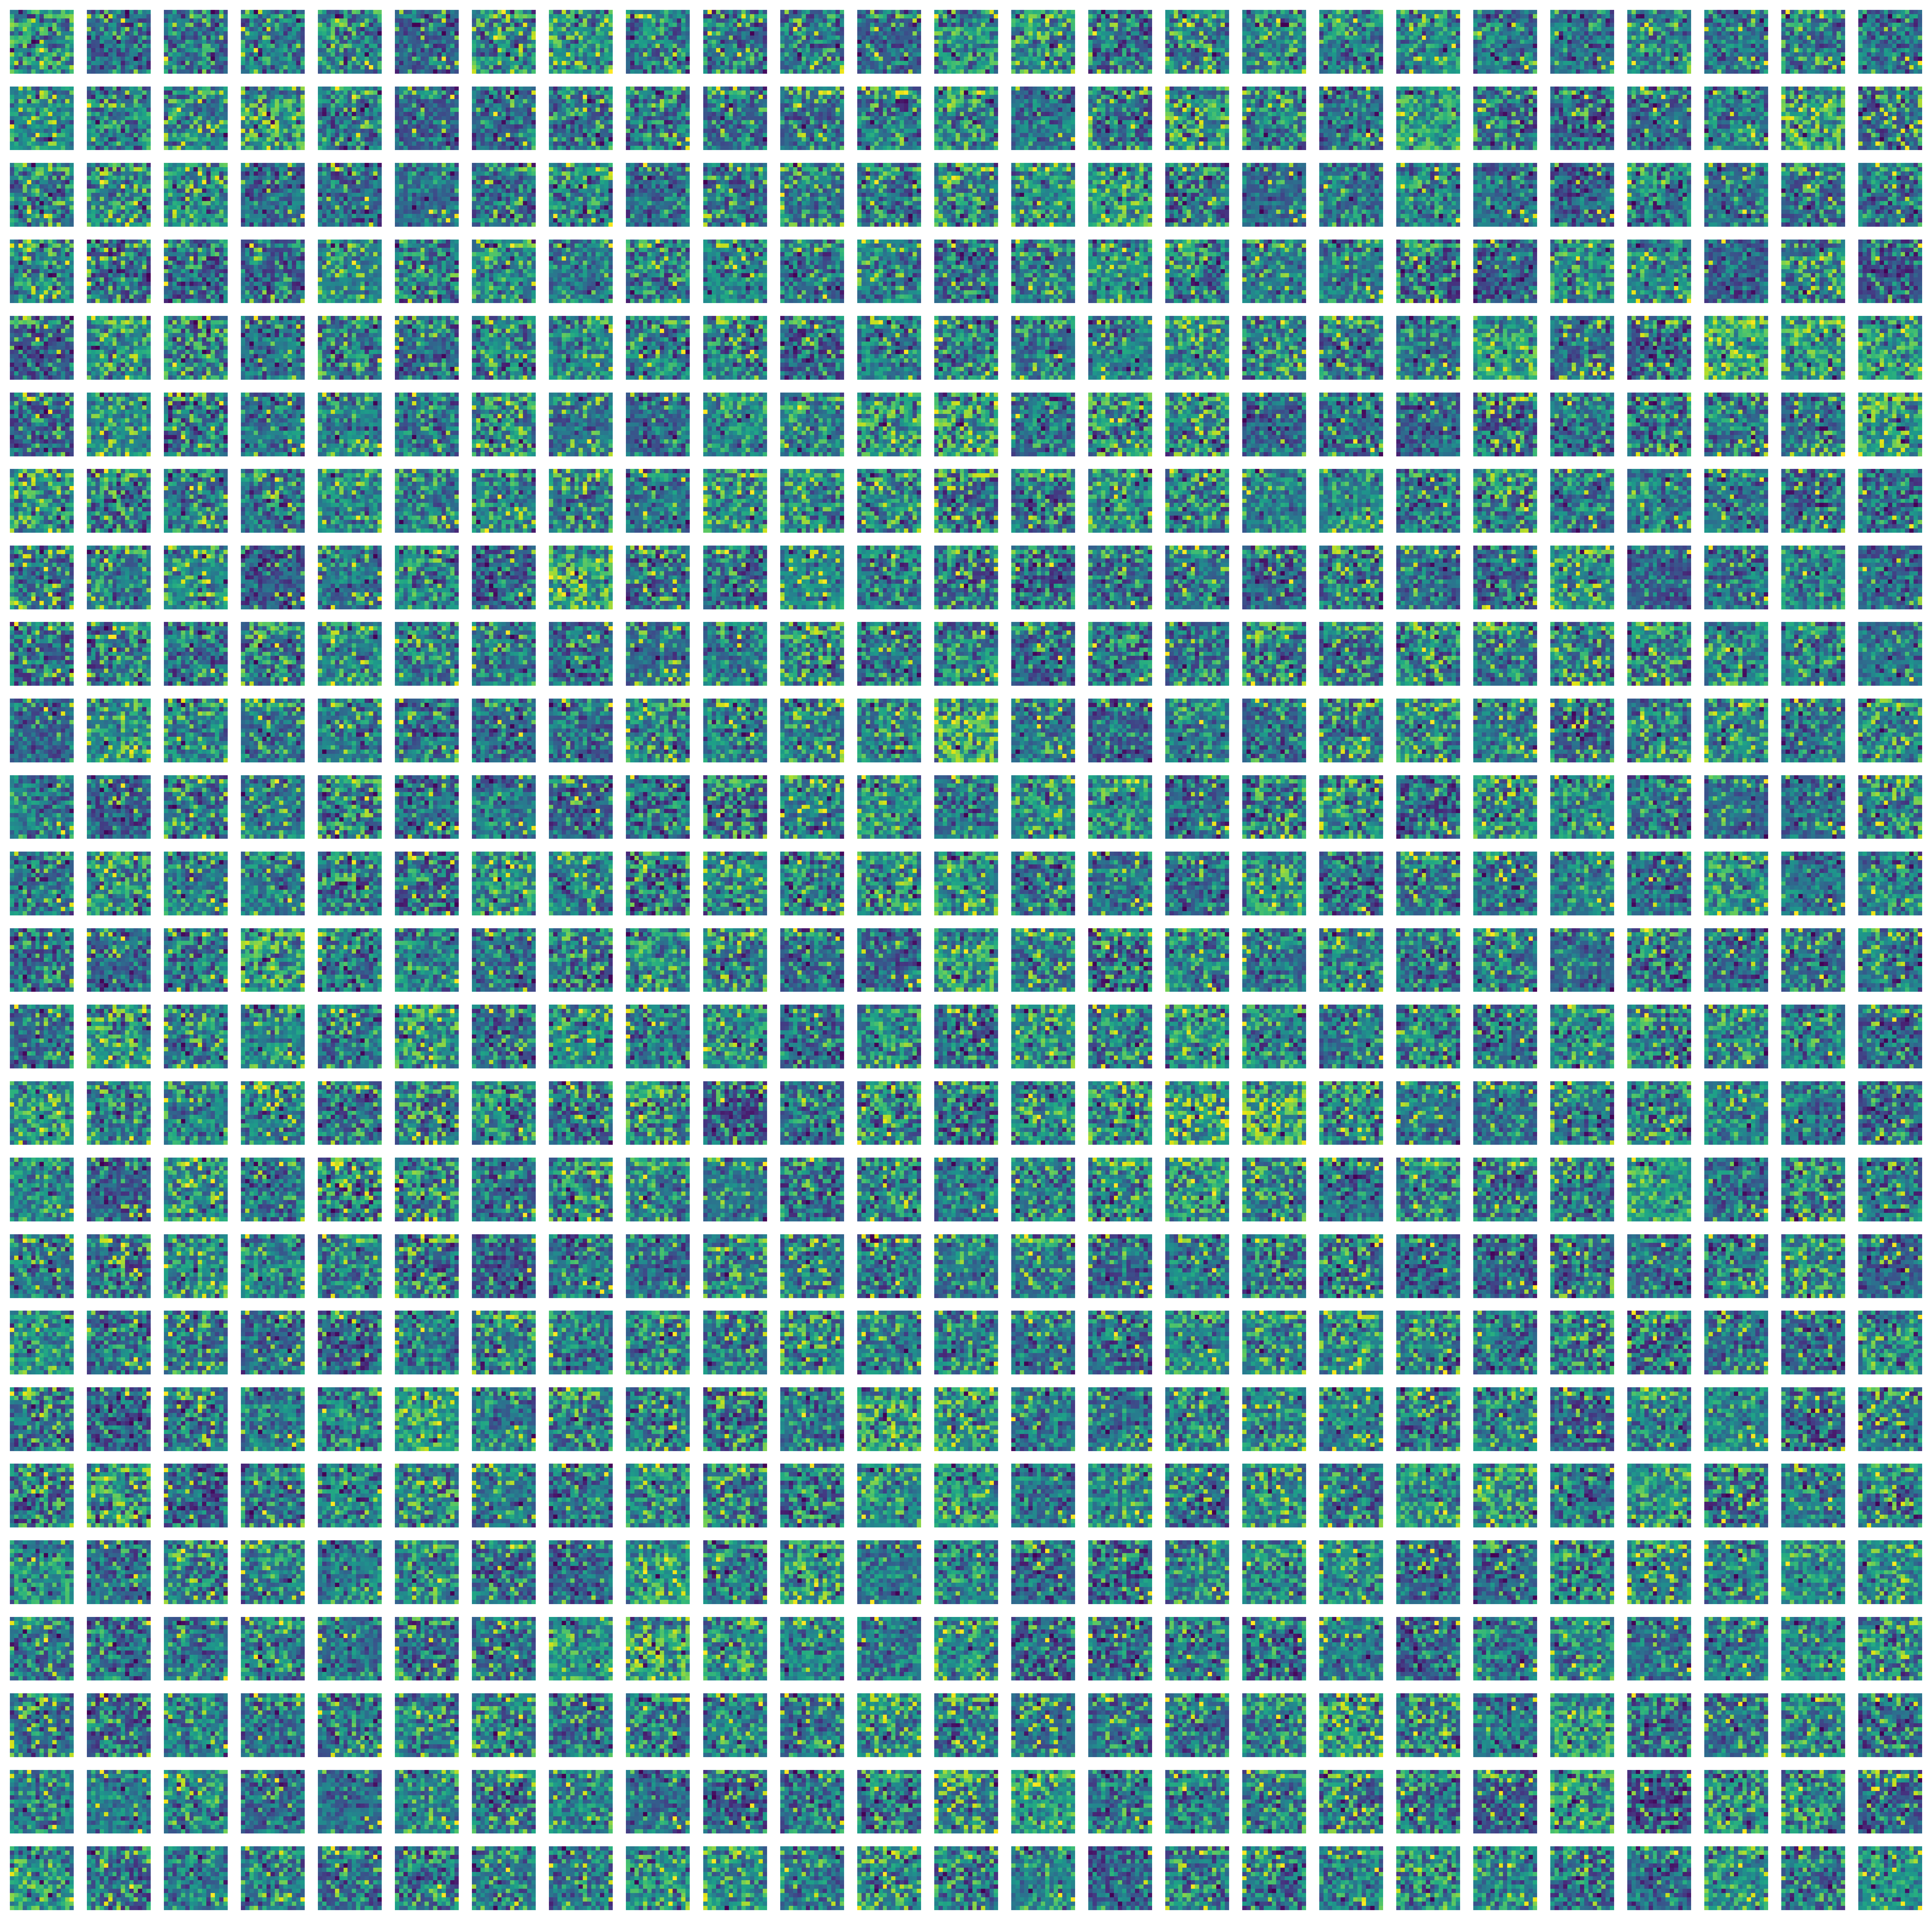
\includegraphics[width=0.3\linewidth]{chapter3/FMs/FMs_RGB_convs_2.png}}

    %  \subcaptionbox
    %     {$FM^{gray}_0$
    %     \label{fig:FM_gray_0}}
    %     {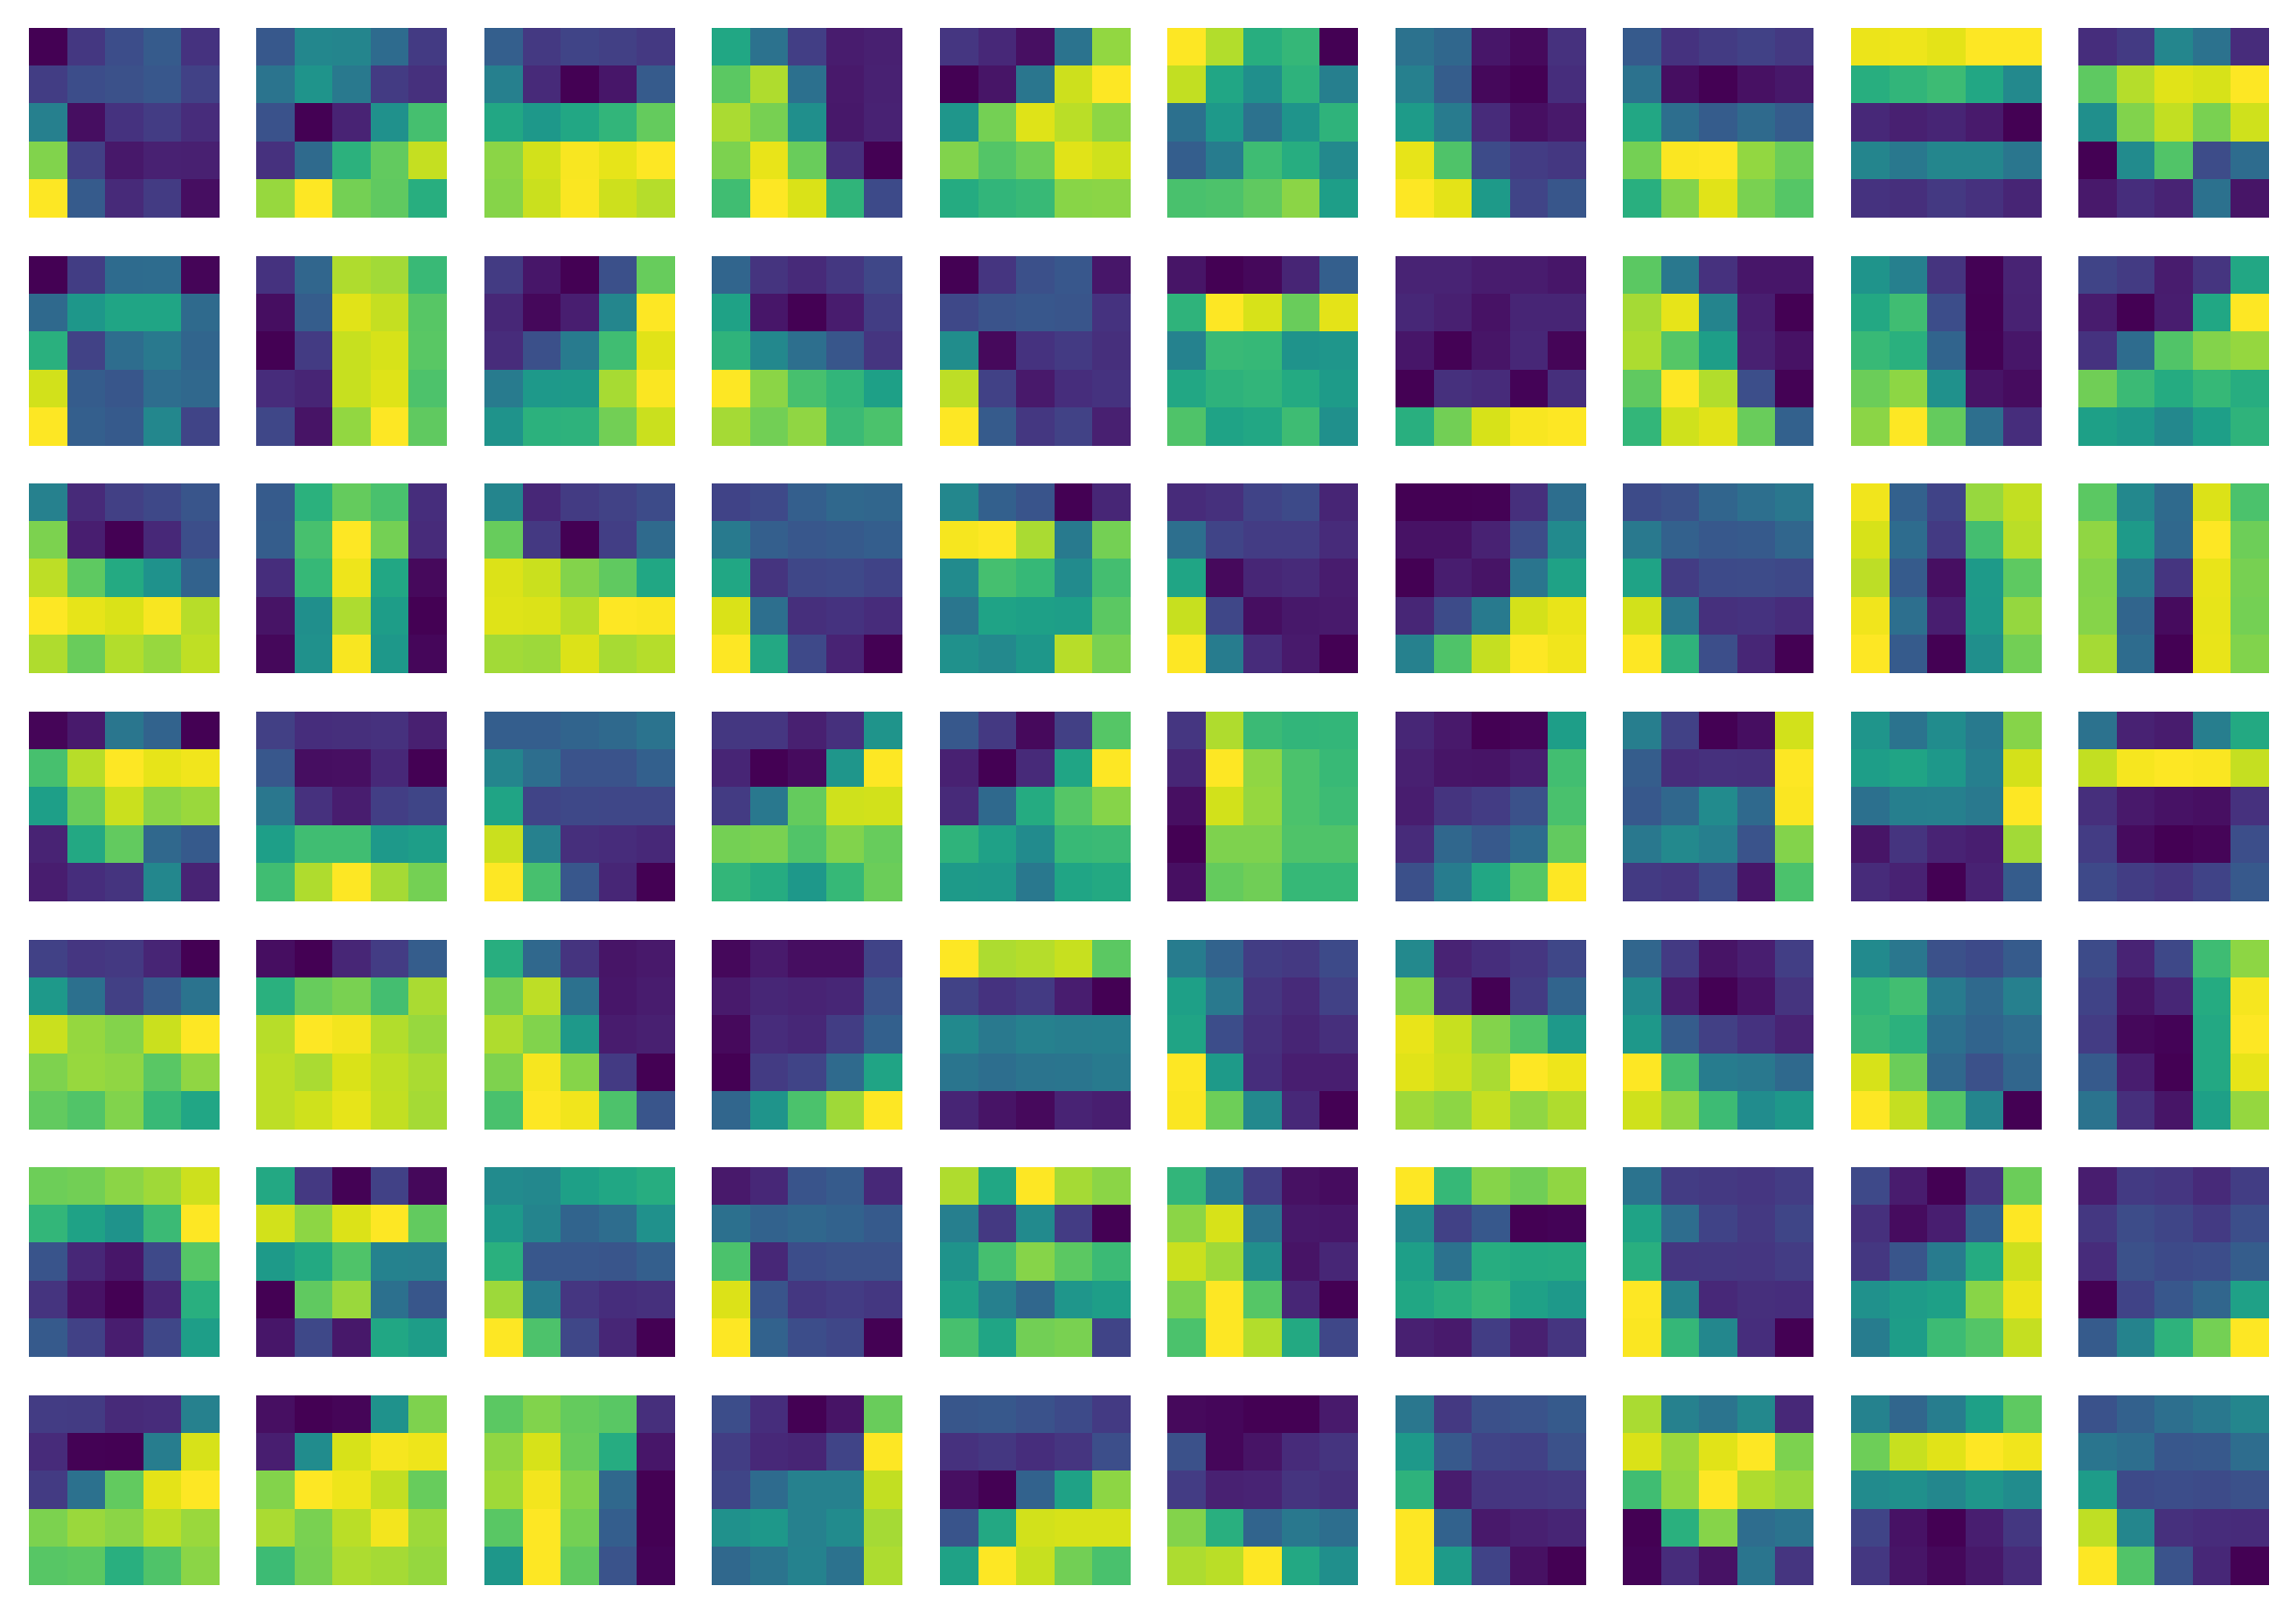
\includegraphics[width=0.3\linewidth]{chapter3/FMs/FMs_Gray_convs_0.png}}
    % ~
    % \subcaptionbox
    %     {$FM^{gray}_1$
    %     \label{fig:FM_gray_1}}
    %     {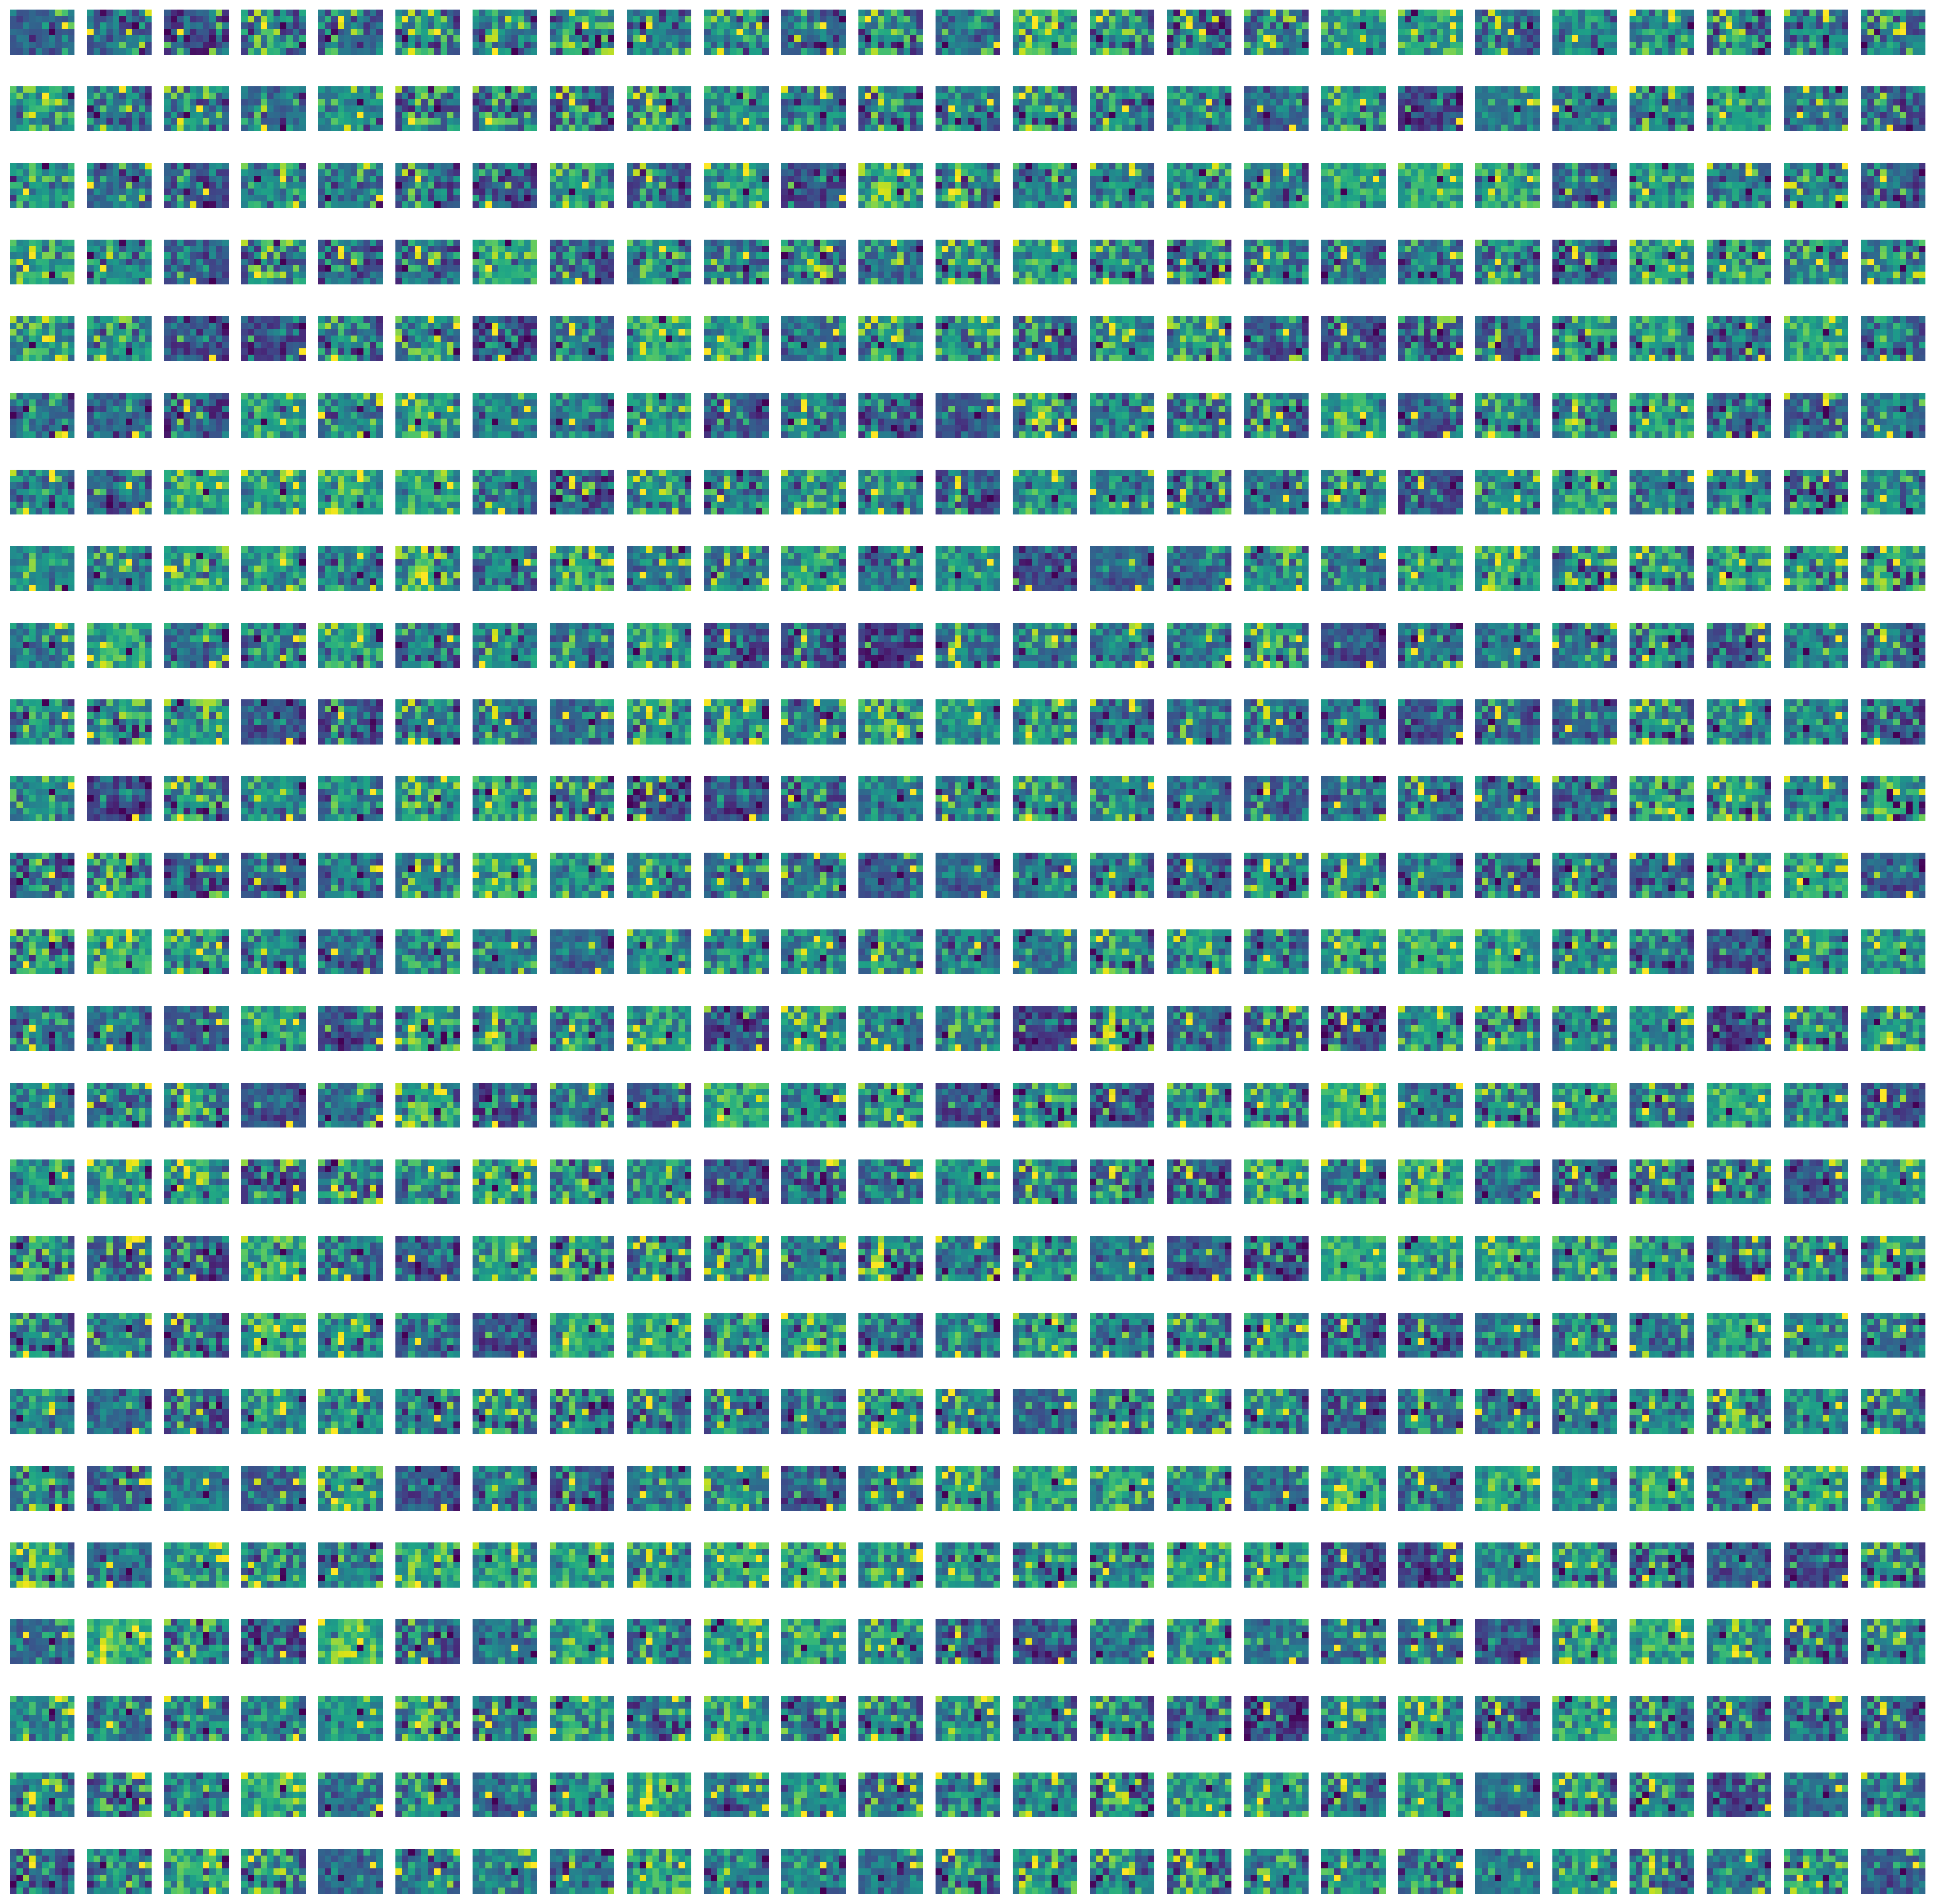
\includegraphics[width=0.3\linewidth]{chapter3/FMs/FMs_Gray_convs_1.png}}
    % ~
    % \subcaptionbox
    %     {$FM^{gray}_2$
    %     \label{fig:FM_gray_2}}
    %     {\includegraphics[width=0.3\linewidth]{chapter3/FMs/FMs_Gray_convs_2.png}}
    % \caption{架構中各層的FM範例}
    % \label{fig:FMs}
	% \end{figure}

	% 特徵映射響應圖(RM)為當輸入進入卷積模組後所得到的輸出進行維度轉換後的結果,
	% 其代表的是輸入區域對於該高斯卷積模組的濾波器的相似度,
	% 也被視為輸入對該高斯卷機模組所有的濾波器的反應強度。
	% 同一層、不同位置的RM數值為輸入影像的不同位置對於某個濾波器的反應,
	% 不同層、同一位置的RM數值為輸入影像的同一位置對於不同濾波器的反應。

	特徵映射圖之對應影像(CI)為記錄資料集中所有影像對特定濾波器的反應,
	從中選出與該濾波器有最大的反應的影像,
	並該影像視為該濾波器的對應影像。
	會需要CI的原因在於除了顏色感知區塊和輪廓感知區塊之外,
	後續的特徵傳遞區塊的輸入均為前一區塊所計算出來的相似度,
	人類已無法去解讀出FM的意義。
	因此我們需要透過CI來找出該濾波器與何種影像最相似,
	幫助使用者理解FM代表的特徵長相。
	每一個區塊每一層的高斯卷積模組的濾波器都會有屬於自己的對應CI影像。
	產生CI的流程如下:
	\begin{itemize}
		\item [1]
		決定要產生CI的目標濾波器
		\item [2]
		將訓練資料集所有影像按照感知區塊之卷積模組的Filter大小進行分割
		\item [3]
		將所有資料集影像輸入進模型,並且記錄目標濾波器所有的輸出
		\item [4]
		選出目標濾波器所有的輸出的最大值,並且找出該最大值的位置
		\item [5]
		選擇該位置在分割影像中的對應小圖
		\item [6]
		分析在目標濾波器所屬的高斯模組前是否有經過空間合併模組。\\
		如果有,則將分割影像按照空間合併範圍進行合併作為目標濾波器的對應CI
	\end{itemize}


	\begin{figure}[H]
	\centering
	\label{fig:CI_generator_0}
	\captionsetup{justification=centering}
	\caption{色彩感知區塊與輪廓感知區塊的CI產生流程示意圖 \\ 以輪廓感知區塊的高斯卷積模組為例}
	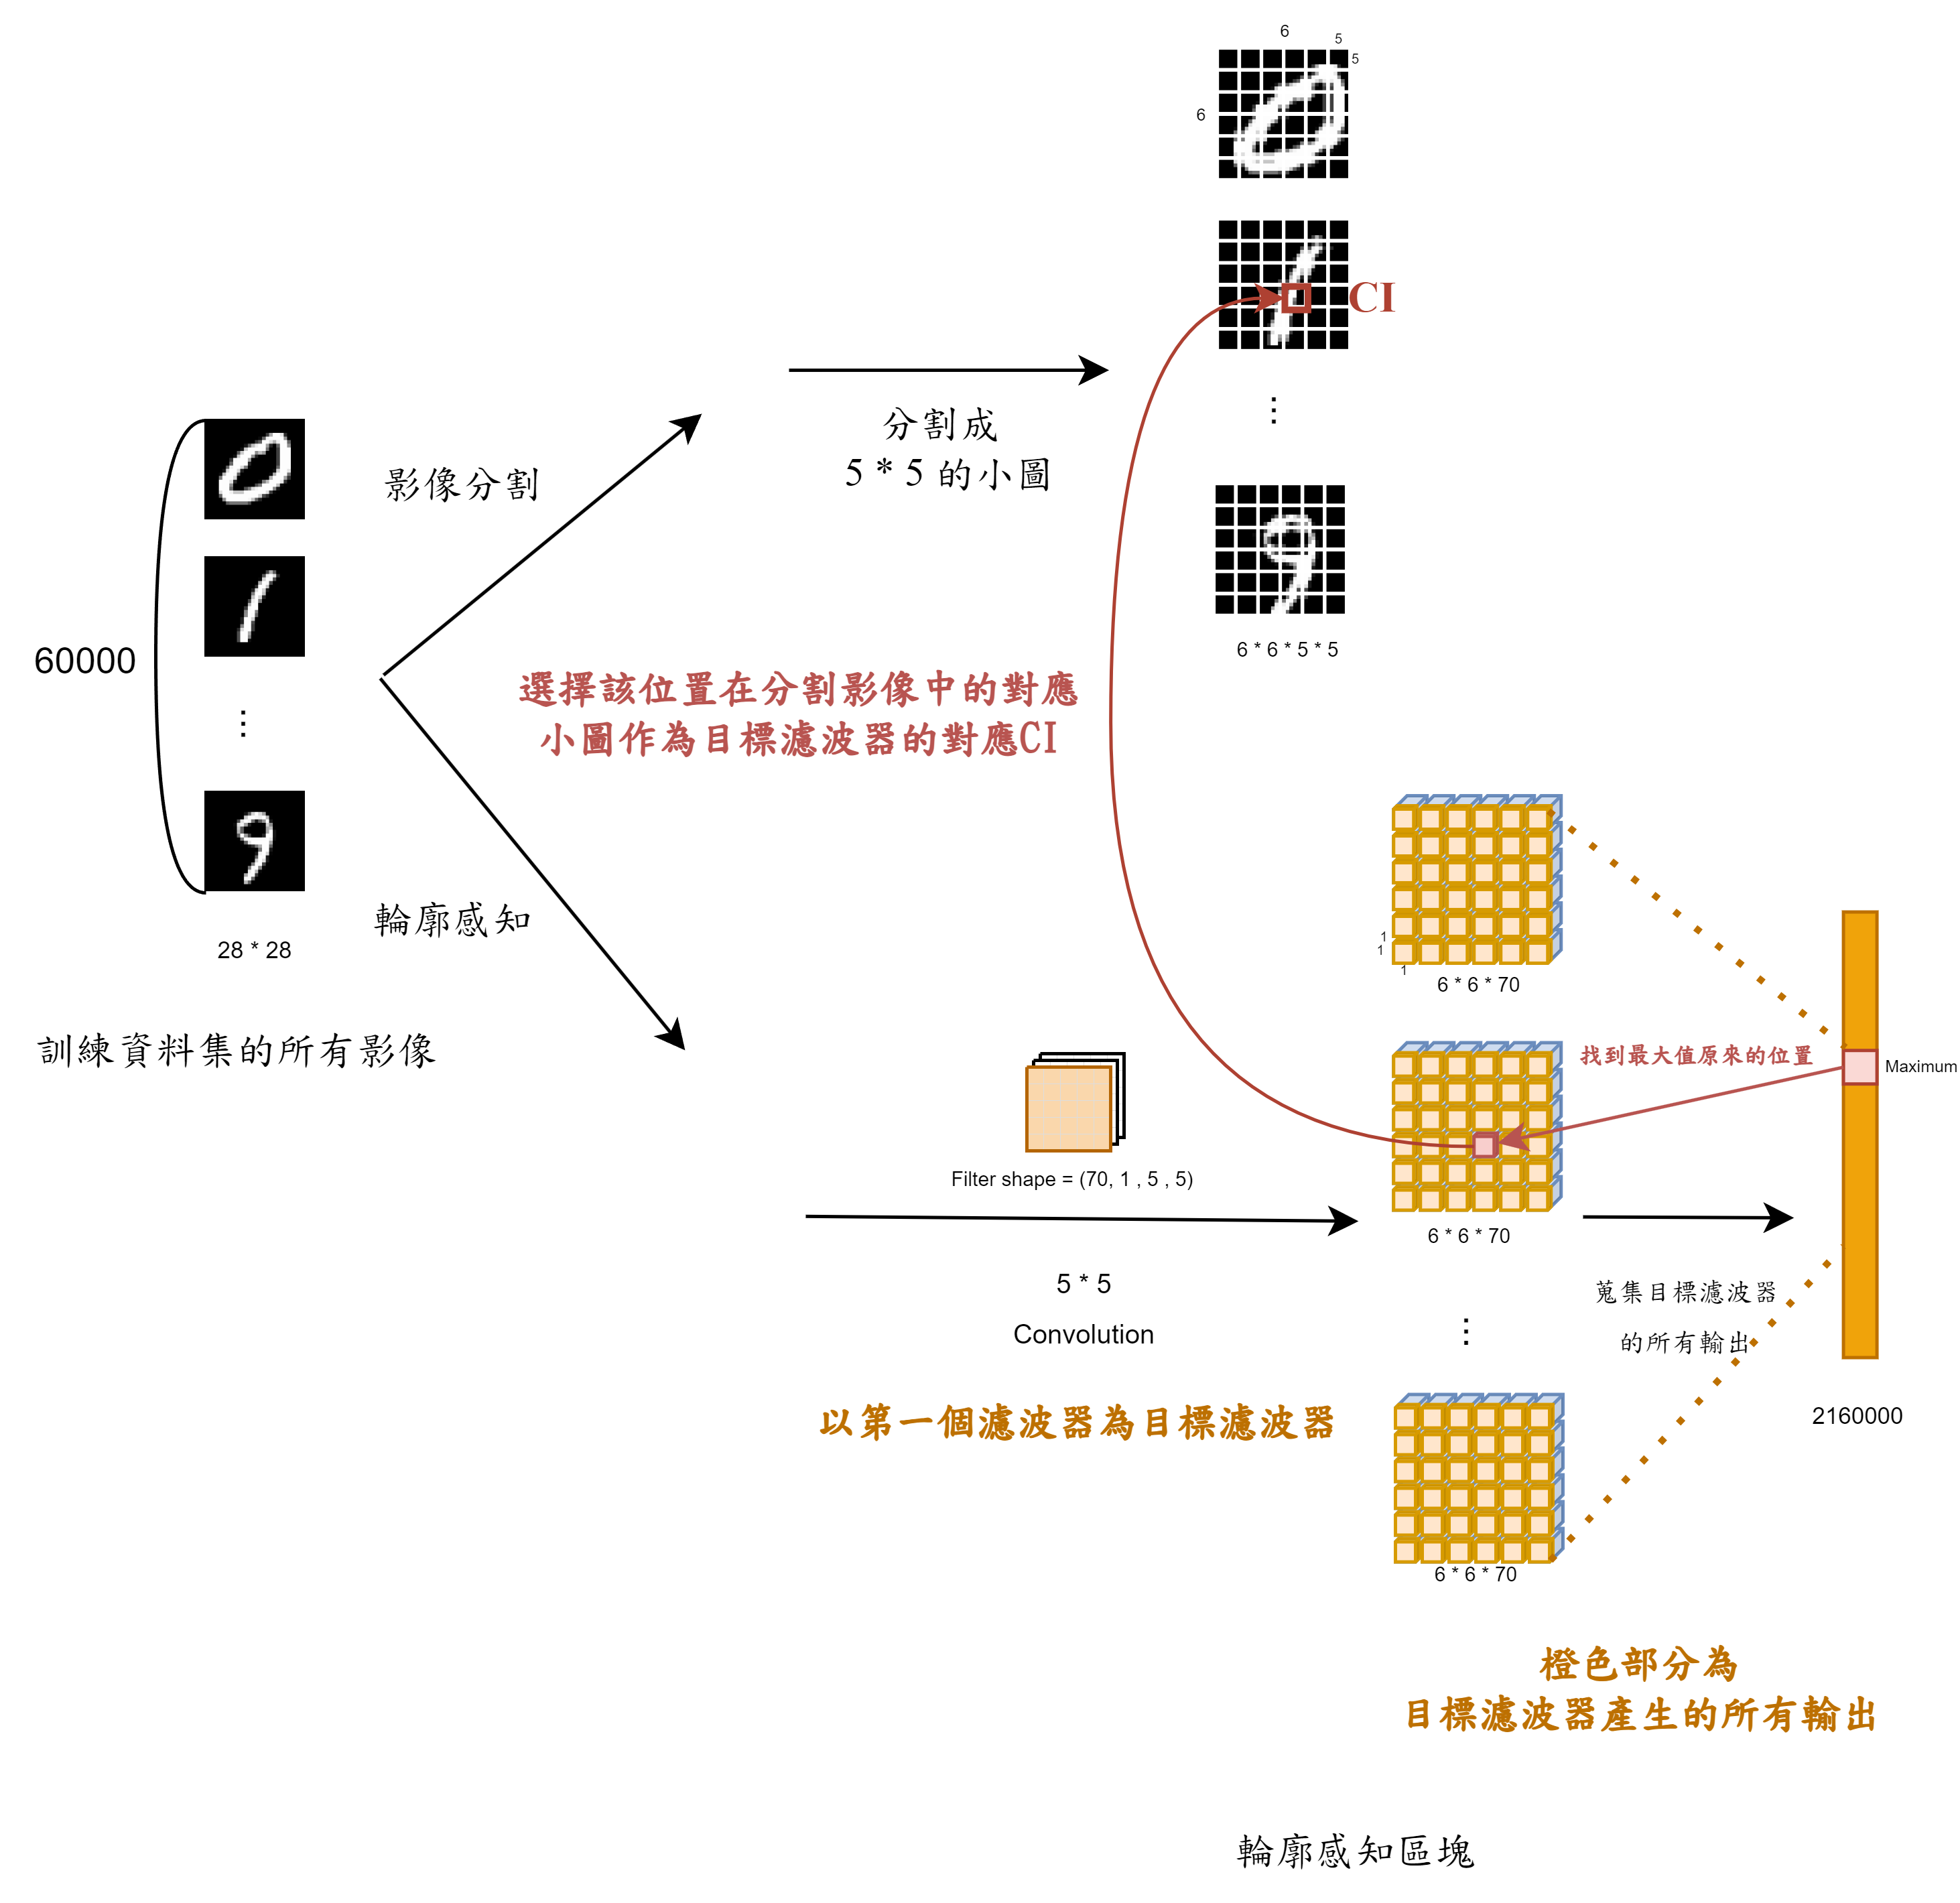
\includegraphics[width=1\textwidth]{chapter3/CI_genenrator_0.png}
	\end{figure}

	\fig[1][fig:CI_generator_1][H]{chapter3/CI_genenrator_1.png}[特徵傳遞區塊之CI產生流程示意圖 \\
	以輪廓特徵傳遞區塊的第一層為例][特徵傳遞區塊之CI產生流程示意圖]

	\begin{figure}[H]
    \centering
    \subcaptionbox
        {$CI^{color}_0$
        \label{fig:CI_color_0}}
        {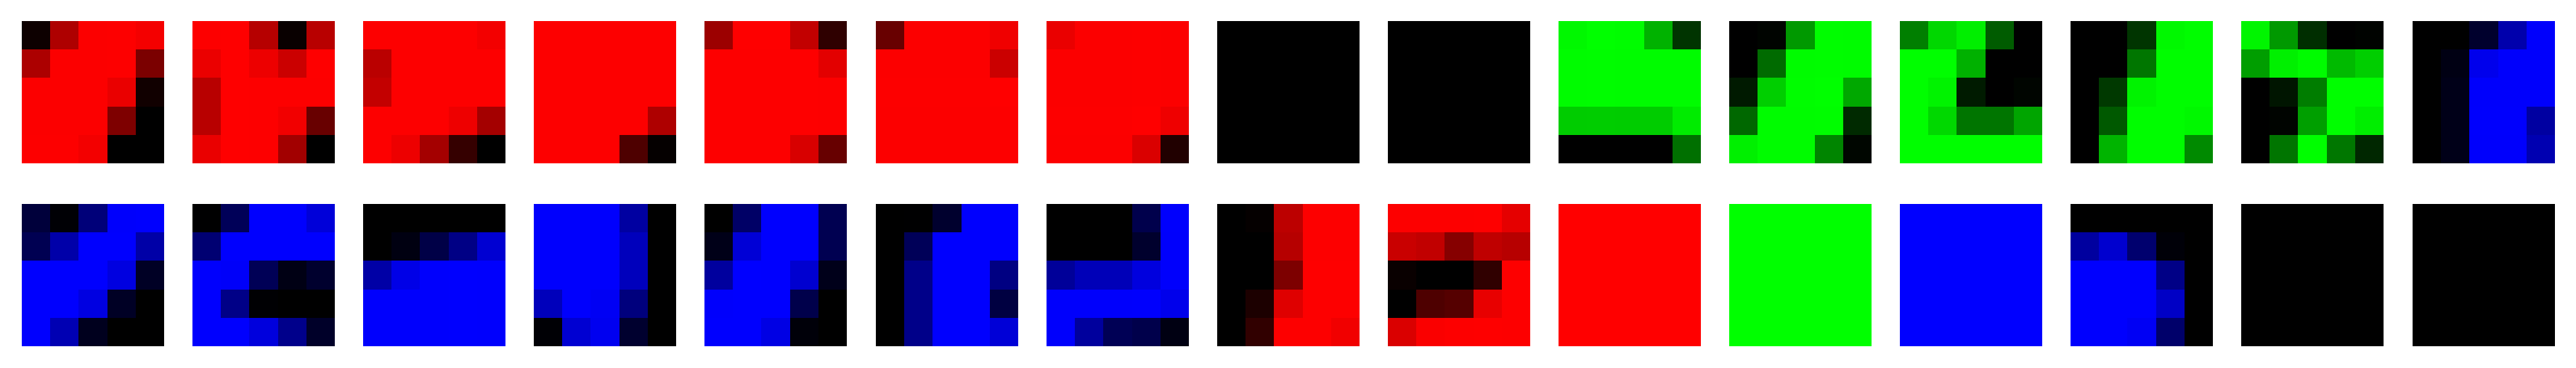
\includegraphics[width=0.3\linewidth]{chapter3/CIs/CIs_RGB_convs_0.png}}
    ~
    \subcaptionbox
        {$CI^{color}_1$
        \label{fig:CI_color_1}}
        {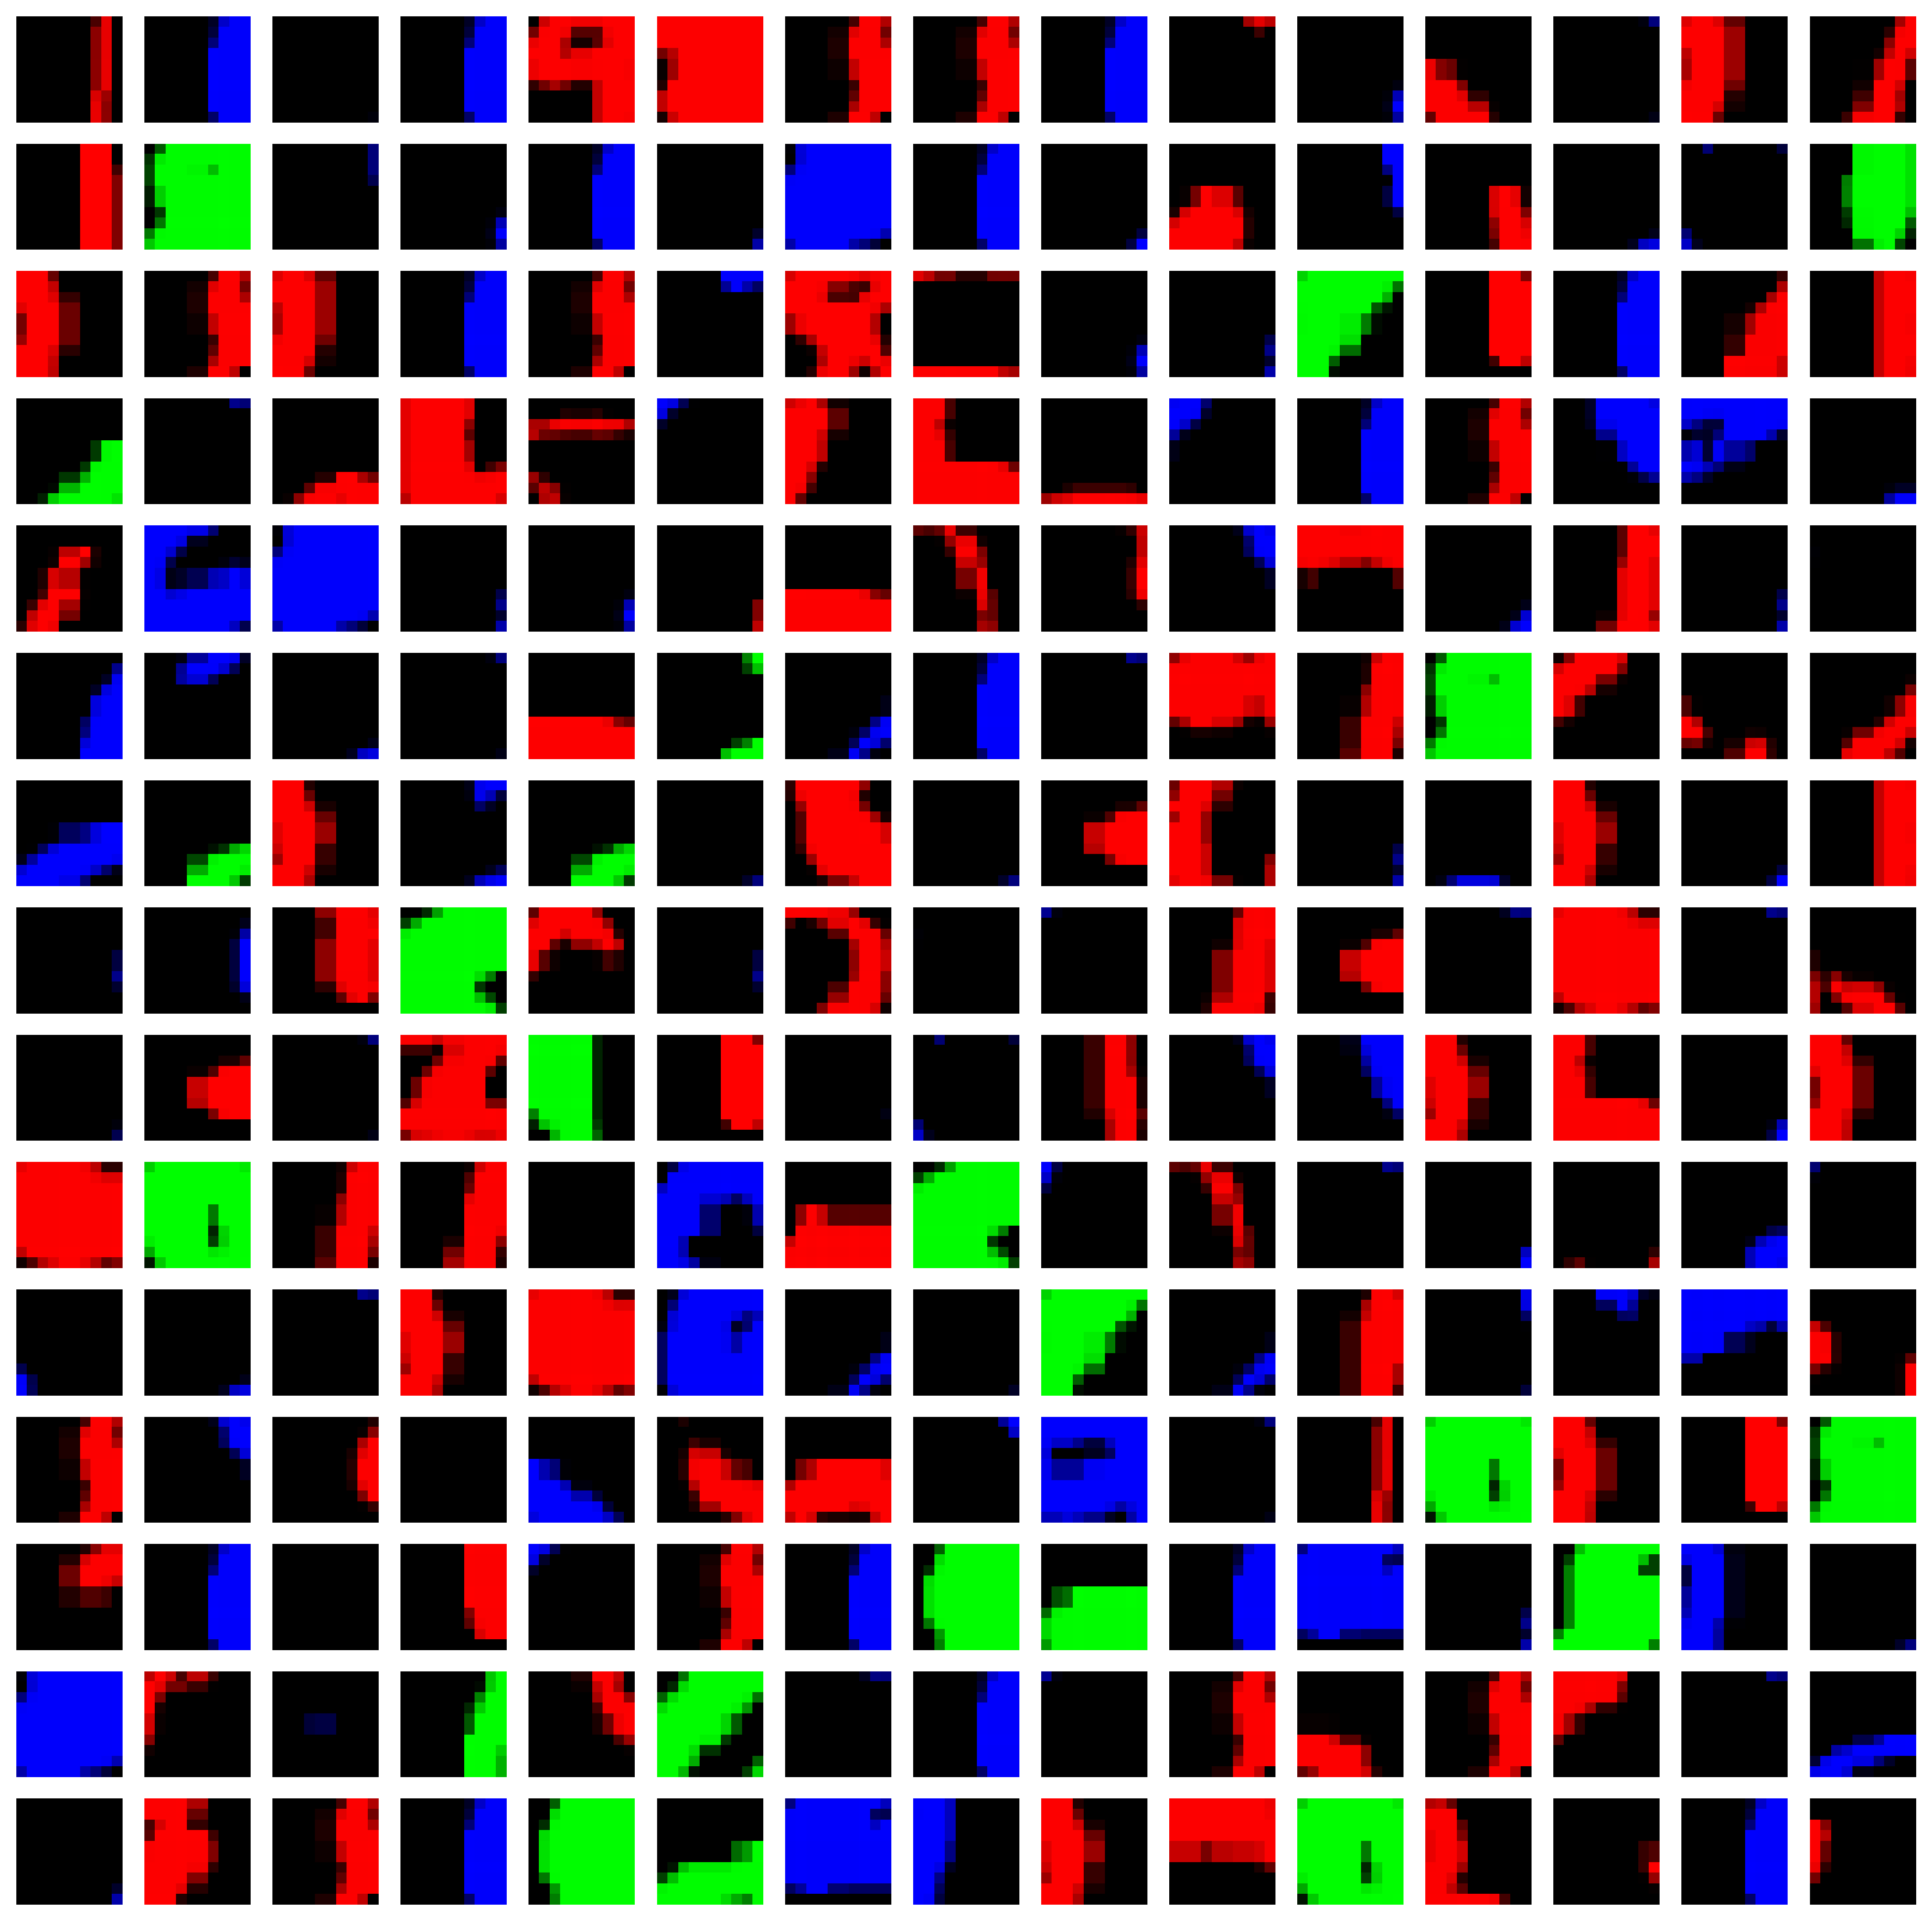
\includegraphics[width=0.3\linewidth]{chapter3/CIs/CIs_RGB_convs_1.png}}
    ~
    \subcaptionbox
        {$CI^{color}_2$
        \label{fig:CI_color_2}}
        {\includegraphics[width=0.3\linewidth]{chapter3/CIs/CIs_RGB_convs_2.png}}

     \subcaptionbox
        {$CI^{gray}_0$
        \label{fig:CI_gray_0}}
        {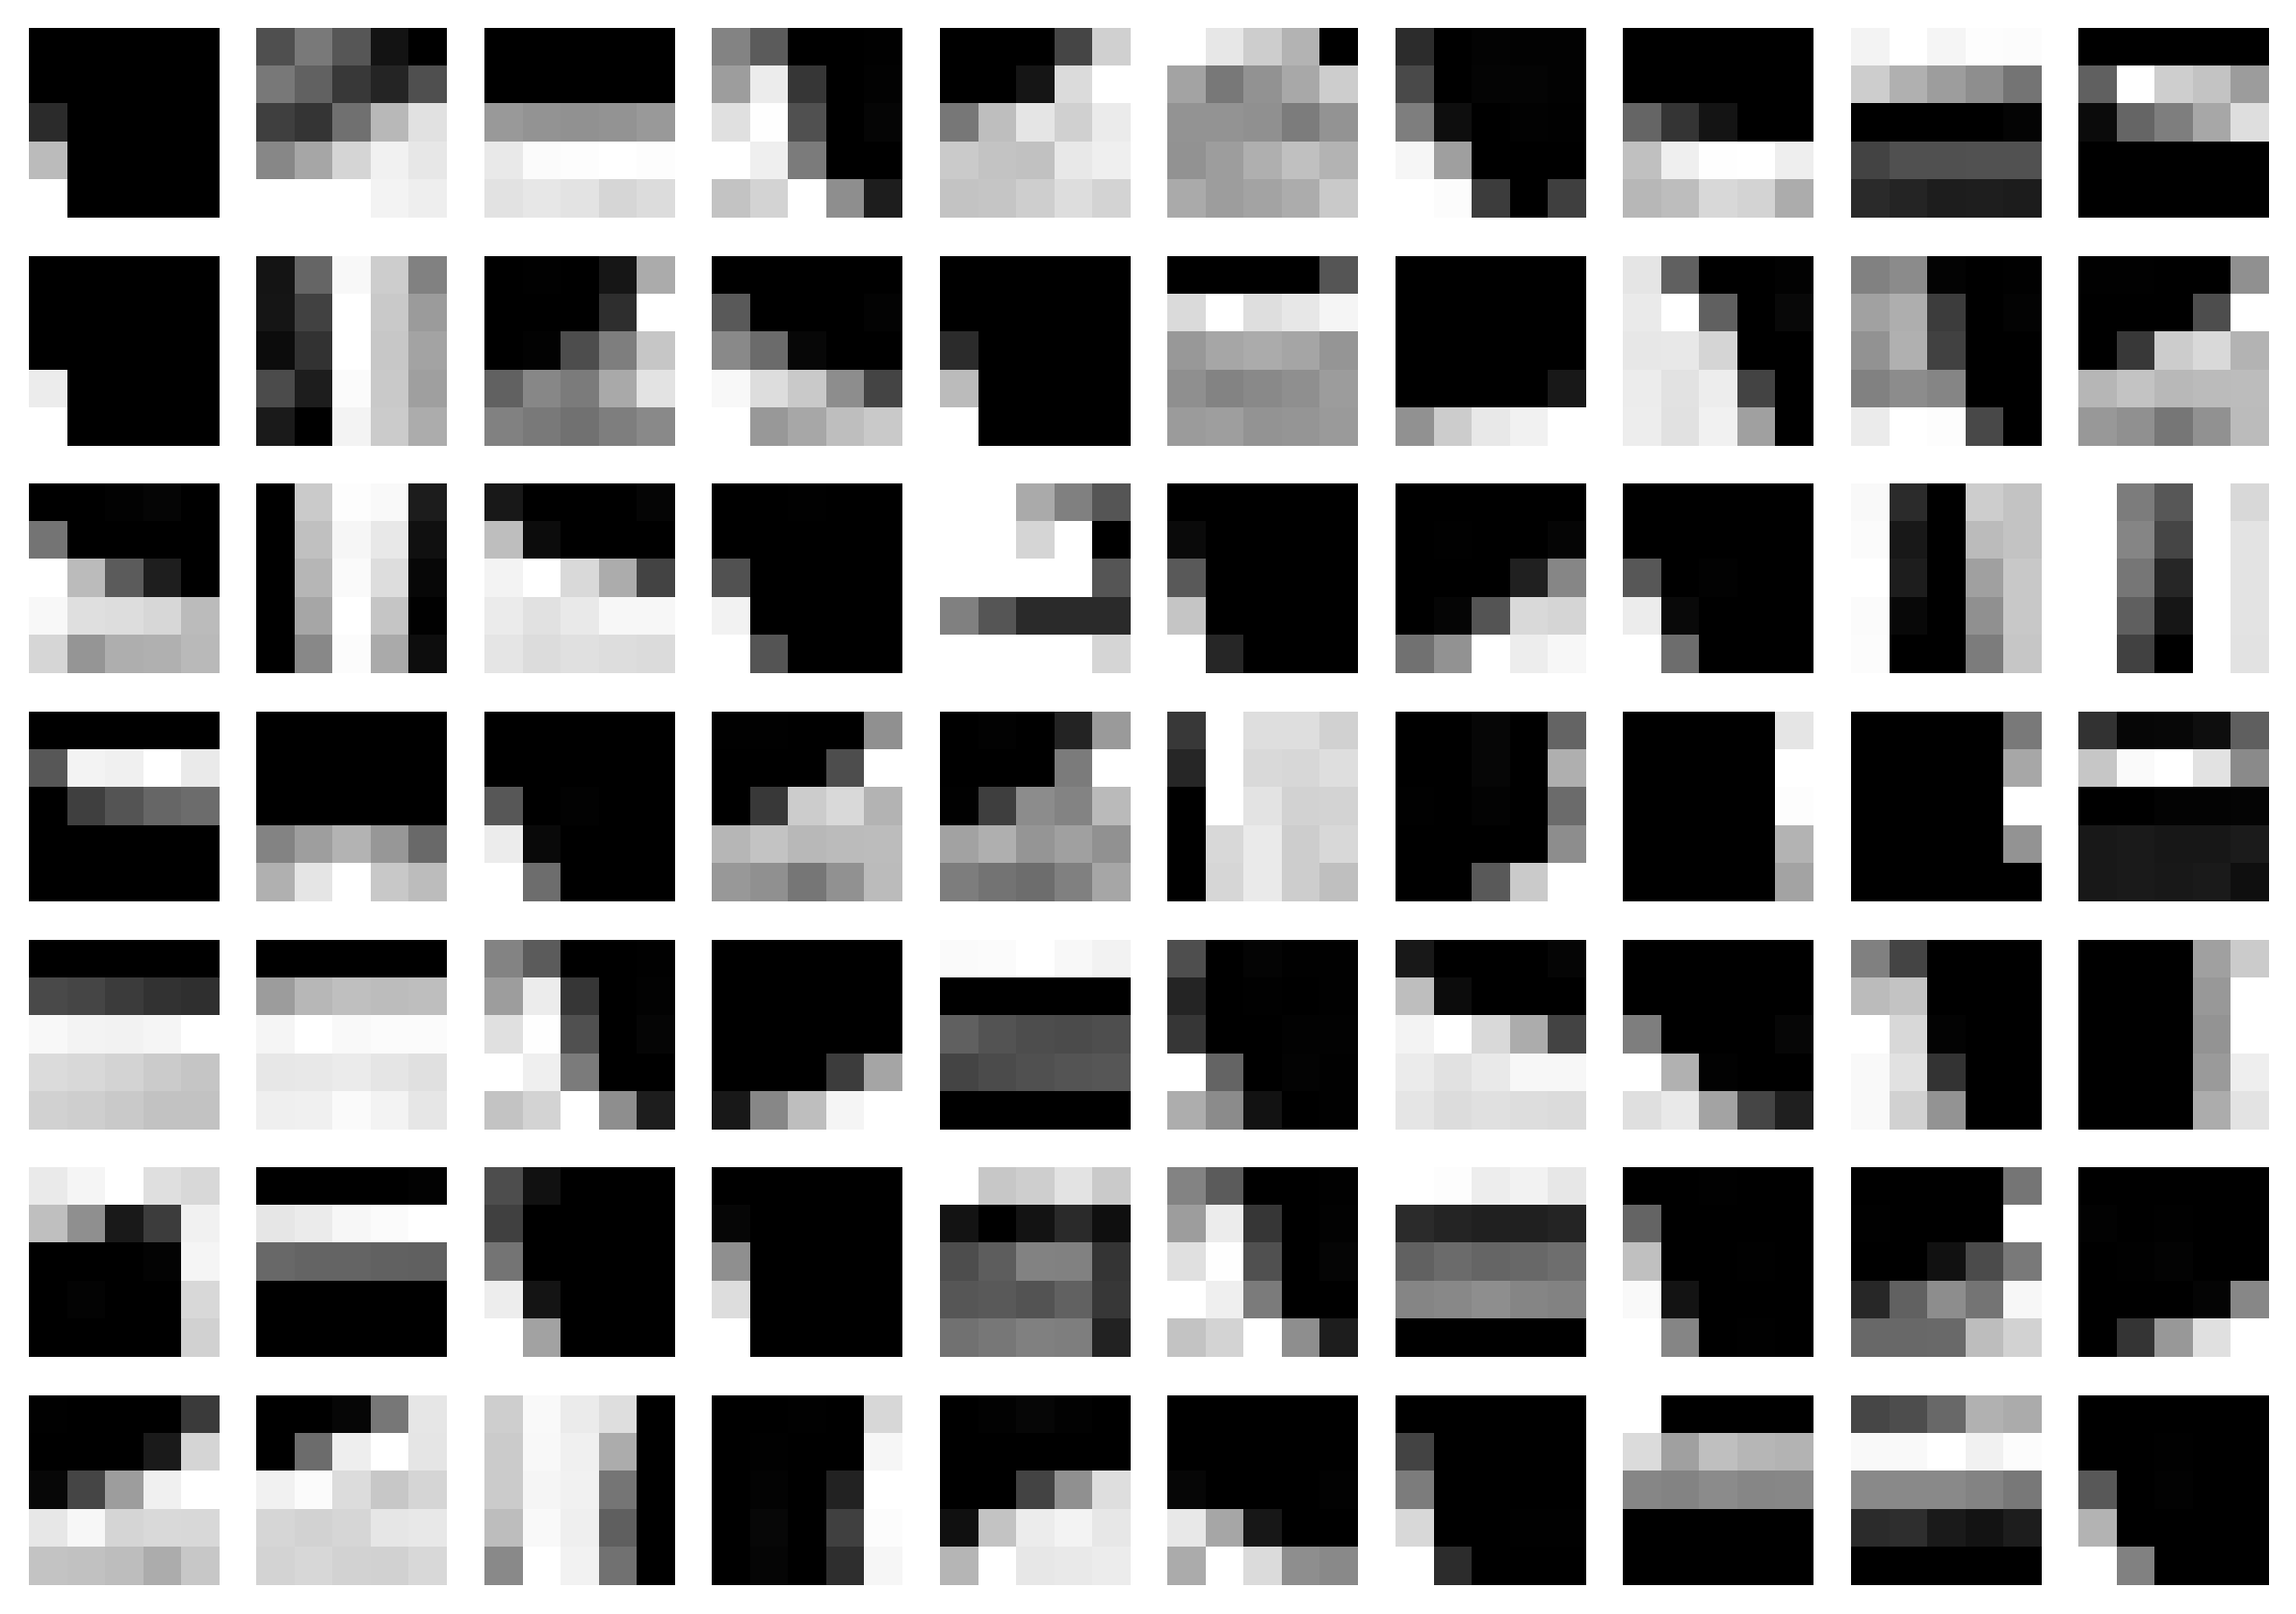
\includegraphics[width=0.3\linewidth]{chapter3/CIs/CIs_Gray_convs_0.png}}
    ~
    \subcaptionbox
        {$CI^{gray}_1$
        \label{fig:CI_gray_1}}
        {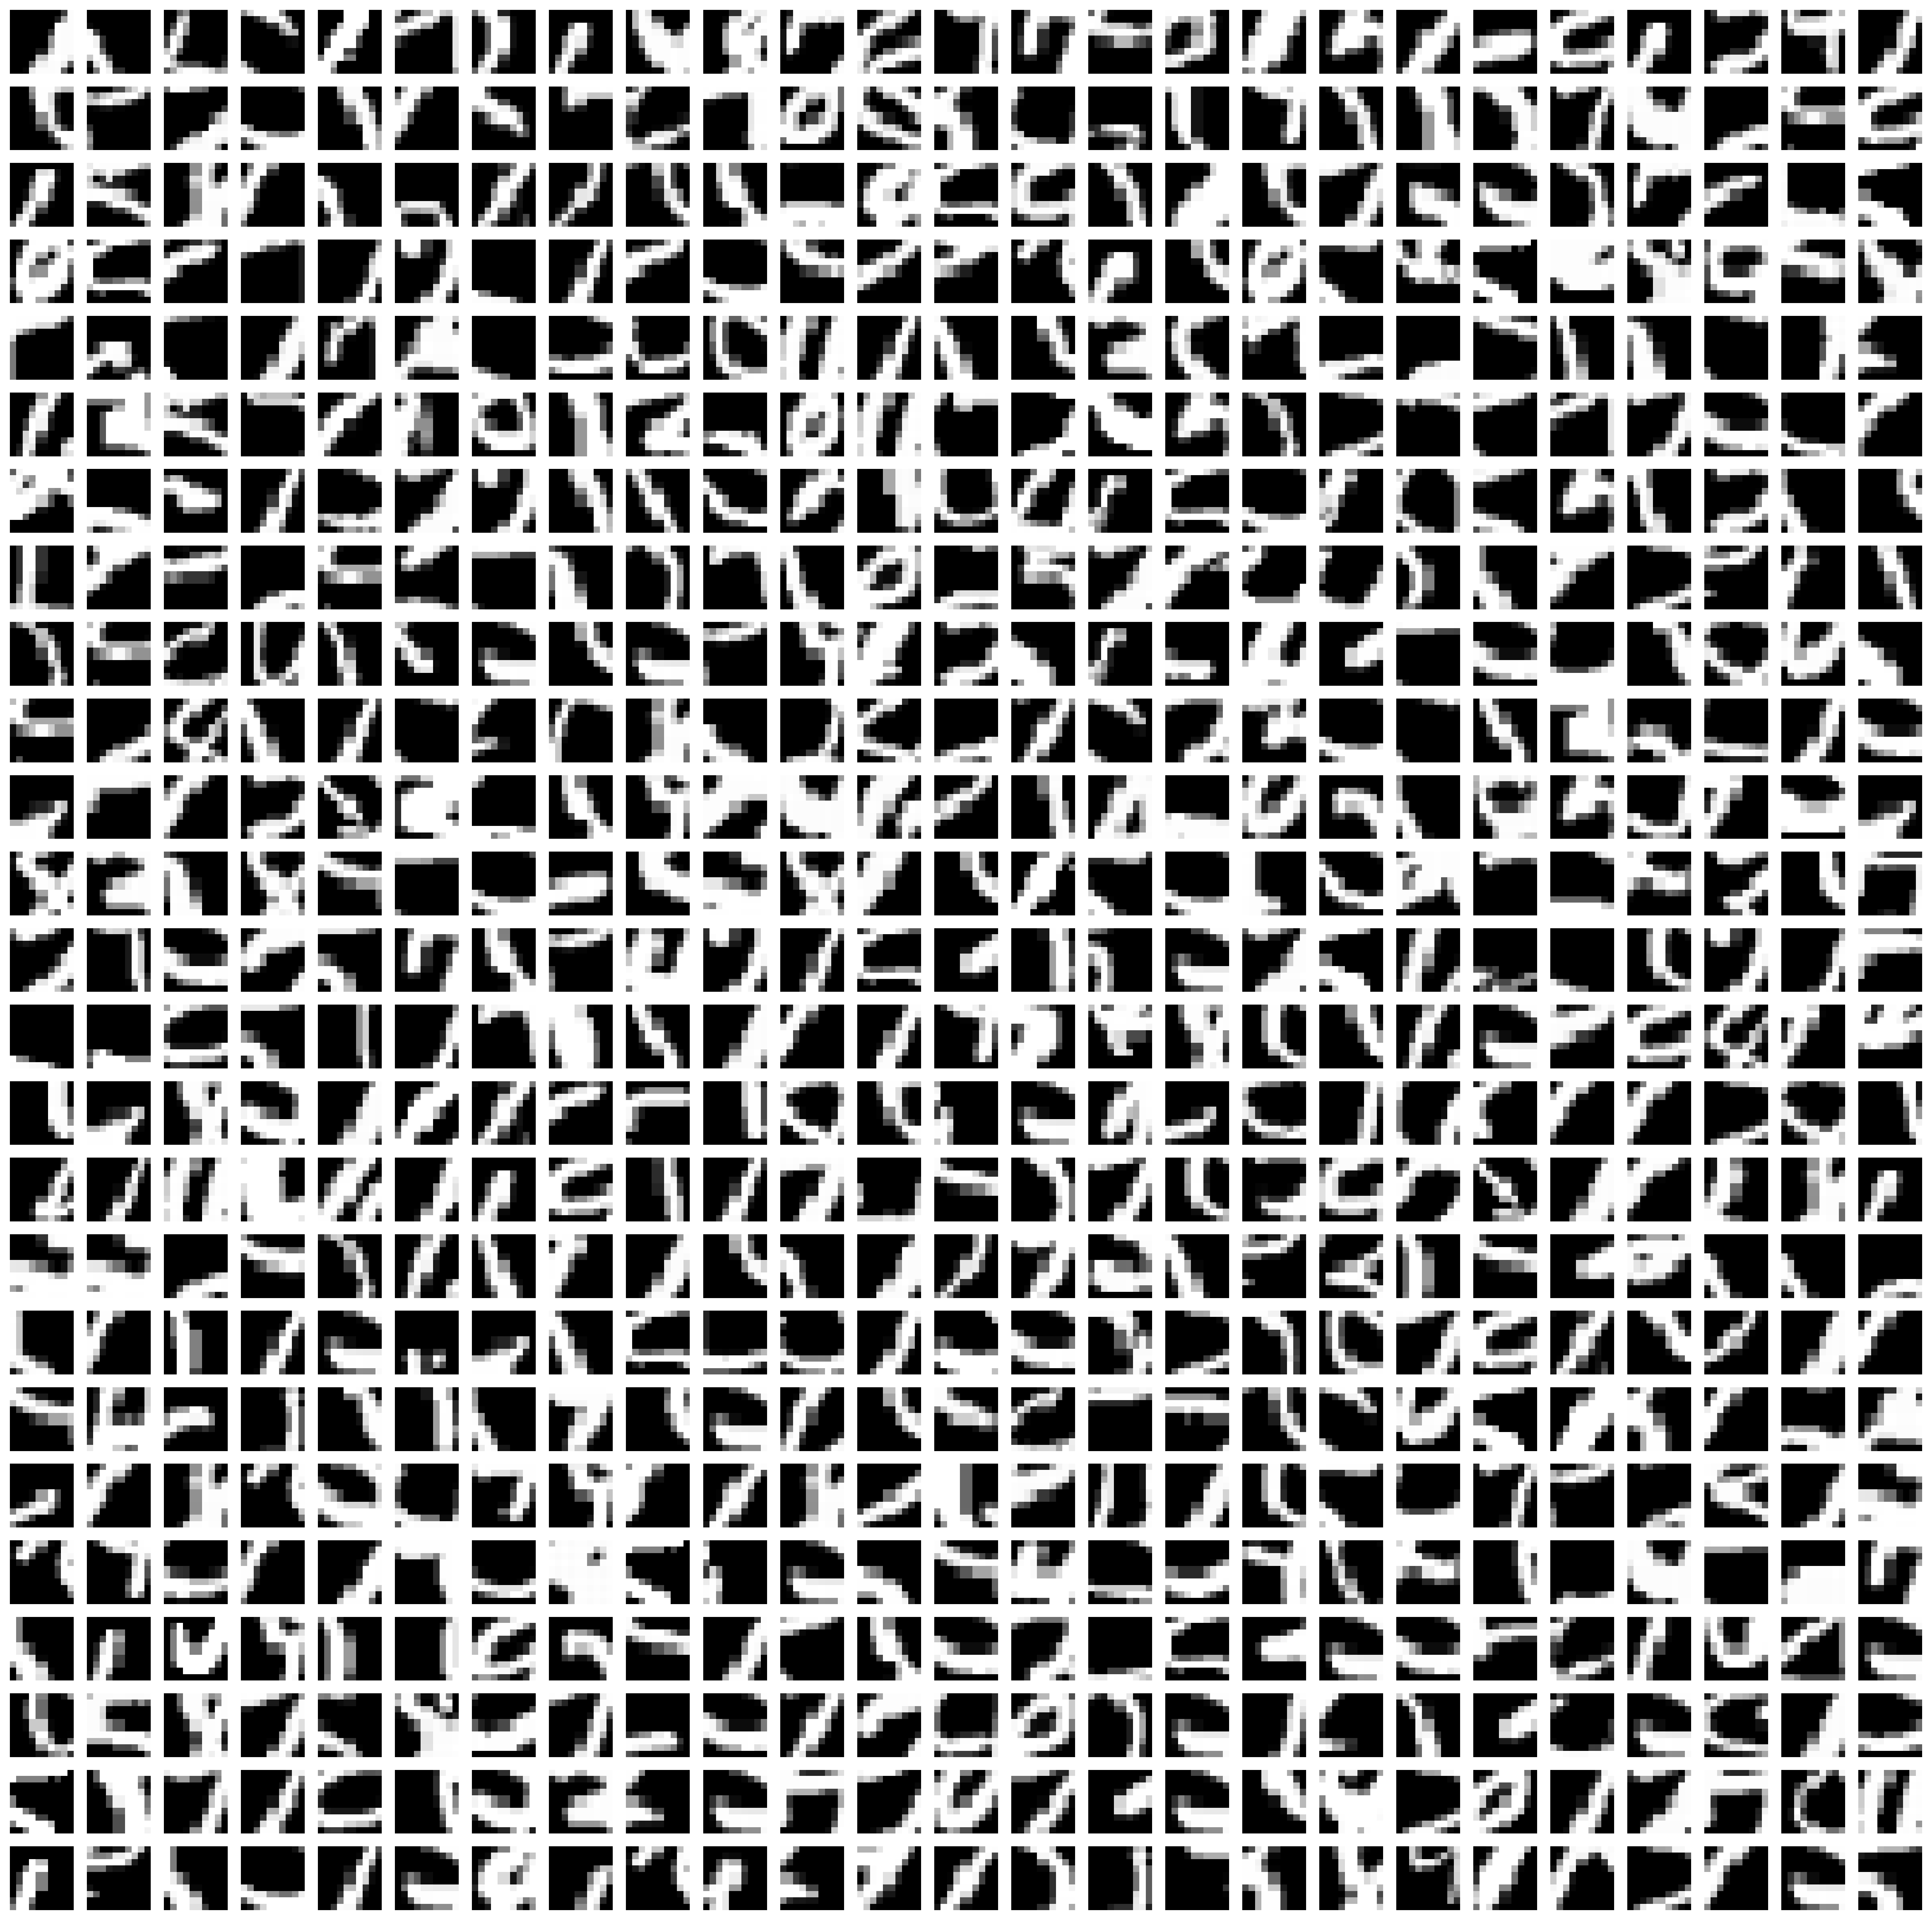
\includegraphics[width=0.3\linewidth]{chapter3/CIs/CIs_Gray_convs_1.png}}
    ~
    \subcaptionbox
        {$CI^{gray}_2$
        \label{fig:CI_gray_2}}
        {\includegraphics[width=0.3\linewidth]{chapter3/CIs/CIs_Gray_convs_2.png}}
    \caption{架構中各層的CI範例}
    \label{fig:CIs}
	\end{figure}

	\pagebreak
	\subsection{色彩感知區塊之視覺化}
	在色彩感知區塊濾波器本身即可被視為 \textit{C}$^{color}_{0}$ 個不同RGB顏色,
	並且這個特性導致FM不會學習到輪廓的特徵。
	然而由於CI是由資料集中影像的部分區塊組成,
	因此FM對應的CI的影像反而卻同時存在顏色和輪廓,
	這會導致最後組合起來導致CI容易出現顏色相似,
	但輪廓與輸入影像完全不同的情況,看起來會十分怪異。
	為了解決這個問題,
	我們會取每個CI的平均色彩作為該CI的代表色,
	我們接著會將CI的代表色擴張為和原始CI相同大小色塊,
	並且使用這些色塊代替原本的CI進行呈現,
	從而更好的反應FM學習到的色彩特徵。

	總結色彩感知區塊產生可解釋性圖片的流程如下:
	\begin{itemize}
		\item [1]
		輸入影像後,找出色彩感應區塊的RM
		\item [2]
		從RM中找出每個RM的最大響應值
		\item [3]
		根據RM的最大響應找出造成響應的濾波器對應的CI
		\item [4]
		找出對應CI的代表色並擴張成與原始CI相同大小的色塊
		\item [5]
		利用色塊組出代表輸入影像各個區域在該層反應最大的濾波器感知到的特徵的影像(RM-CI-Color-0)
	\end{itemize}

	\fig[0.6][fig:RMCI_Color_generator][H]{chapter3/RMCI_Color_generator.png}[色彩感知區塊產生RM-CI流程圖][色彩感知區塊產生RM-CI流程圖]

	\pagebreak

	\subsection{色彩特徵傳遞區塊之視覺化}
	在色彩特徵區塊上,
	由於經過空間合併模組的特徵合併,
	因此該區塊所學到的是比色彩感知區塊更加完整的特徵。
	為了準確地呈現FM對應的CI的不同的顏色與位置,
	我們採用以下的方法進行處理:\\
	首先,我們找到輸入影像在該區塊的高斯卷積模組對應的CI。
	接者,將這些CI切成與$CI_{color}$相同大小的小圖,
	然後,對這些小圖分別取平均顏色並將這些平均顏色擴張為和$CI_{color}$相同大小的色塊,
	用這些色塊代替原本的CI按照對應位置組成RM-CI影像。
	再加入了分割這個步驟後,每個CI都能反映出不同部分對應的顏色和位置,
	從而更好的呈現CI的顏色分布。

	\fig[0.7][fig:Color_CI][H]{chapter3/Color_CI.png}[色彩特徵傳遞區塊產生CI示意圖][色彩特徵傳遞區塊產生CI示意圖]

	總結色彩特徵傳遞區塊產生可解釋性圖片的流程如下:
	\begin{itemize}
		\item [1]
		輸入影像後,找出色彩感應區塊的RM
		\item [2]
		從RM中找出每個RM的最大響應
		\item [3]
		根據RM的最大反應位置找出造成響應的濾波器對應的CI
		\item [4]
		將對應的CI分割成數個與$CI_{color}$相同大小的小圖
		\item [5]
		找出各個小圖的代表色並擴張成與原始CI相同大小的色塊
		\item [6]
		利用色塊組出代表輸入影像各個區域在該層反應最大的濾波器感知到的特徵的影像(RM-CI-Color-i),i 為區塊的第i層
	\end{itemize}

	\fig[1][fig:RMCI_color_transfer][H]{chapter3/RMCI_color_transfer.png}[色彩特徵傳遞區塊產生RM-CI流程圖][色彩特徵傳遞區塊產生RM-CI流程圖]
	\pagebreak

	\subsection{輪廓感知區塊和輪廓特徵傳遞區塊之視覺化}
	輪廓感知和特徵傳遞區塊的可解釋性採用的是CIM的特徵圖對應法,
	利用輸入影像在每層的高斯卷積模組的RM,從RM中選出最大的反應強度,
	根據反應強度的位置找出對應的CI,並組出輸入影像在該層的代表影像。

	總結輪廓感知區塊和輪廓特徵傳遞區塊產生可解釋性圖片的流程如下:
	\begin{itemize}
		\item [1]
		輸入影像後,找出色彩感應區塊的RM
		\item [2]
		從RM中找出每個RM的最大反應
		\item [3]
		根據RM的最大反應位置找出對應的CI
		\item [4]
		利用CI組出能夠代表輸入影像各個區域在該層反應最大的濾波器感知到的特徵的影像(RM-CI-Gray-i),i 為特徵傳遞區塊的第i層,第0層為輪廓感知區塊
	\end{itemize}

	\fig[0.7][fig:RMCI_gray][H]{chapter3/RMCI_gray.png}[輪廓感知區塊和輪廓特徵傳遞區塊產生RM-CI流程圖 \\ 
	以輪廓感知區塊為例][輪廓感知區塊和輪廓特徵傳遞區塊產生RM-CI流程圖]

\pagebreak

	\subsection{RM-CI的可解釋性}
	根據上面視覺化流程,
	當我們產出輸入影像在每層的代表影像,也就是每層的RM-CI的時候,
	我們就可以針對每層的RM-CI進行解釋。
	RM-CI的定義為由輸入影像的每個區塊在某層的卷積模組中的最大響應濾波器的對應影像所組成的影像,
	其代表了模型在該層感知到輸入影像的每一個區塊的特徵,
	透過每層的RM-CI的不斷形成,
	我們可以觀察出模型在輸入影像的不同位置不同大小區域感知到了哪些特徵,
	並且也可以解釋模型在每層的卷積模組中是由於看到了哪些特徵才做出最後的預測。

	以\cref{fig:Explain_example}為例,
	我們從 RM-CI-Color-2 和 RM-CI-Gray-2 中我們可以解釋出,
	模型特徵傳遞區塊的最後一層是因為看到影像的上面部分有一個下彎弧,
	中間部分有曲線向下,下面部分有上彎弧,
	配合上在三個部分都有看到綠色,所以才判斷影像為綠色的0。
	而模型會認為影像的上面部分要有下彎弧的依據是因為中間部分有斜曲線,
	右上角有另一半斜曲線,組合成一個下彎弧,
	所以才導致模型認為影像的上半部分為下彎弧,
	以此類推。
	我們便可以對依序推出模型的每層的判斷歷程。
	\fig[0.7][fig:Explain_example][H]{chapter3/Explain_example.png}[可解釋性的範例][可解釋性的範例]

\pagebreak

\subsection{全連接層的可解釋性}
本模型全連接層如\cref{fig:Linear}所示,
全連接層的輸入由色彩特徵傳遞區塊的輸出$Ouput^{color}$
和輪廓特徵傳遞區塊的輸出$Ouput^{gray}$所組成,
其全連接層的權重計算公式為\cref{eq:eq-linear},
其中$w_{ji}$為第j個神經元與第i個神經元的權重,
$w_{j0}$為第j個神經元的偏移量,
$K$ 為$Ouput^{color}$經過Flatten後的長度,
$L$ 為$Ouput^{color}$經過Flatten後的長度加上$Ouput^{gray}$經過Flatten後的長度,
$x_{i}$為第i個神經元的輸入,
$y_{j}(x)$為第j個神經元的輸出,
$j$的數量為類別的數量。
\begin{equation}
    \label{eq:eq-linear}
    y_{j}(x) = \sum_{i=1}^{K}w_{ji} * x_{i} + \sum_{i=K+1}^{L}w_{ji} * x_{i} + w_{j0}
\end{equation}

根據上面的公式我們可以發現,
如果某個第j個類別機率越大,則代表$\sum_{i=1}^{L+K}w_{ji} * x_{i}$越大。
利用此特性結合上面所說的$x_{i}$由$Ouput^{color}$和$Ouput^{gray}$組成,
我們在回推時,
便可以將$w_{ji} * x{i}$根據$x$的來源分為兩類。

一類為$x_{i}$屬於$Ouput^{color}$與其對應的$w_{ji}$相乘的$w_{ji} * x{i}$,
其$i$的範圍為1到K之間,
我們將其視為色彩特徵傳遞區塊的RM,
其對應的FM為色彩特徵傳遞區塊最後一層高斯卷積模組的FM,
透過此FM找到對應的CI,由此可視化出色彩上全連接層的權重。
另一類為$x_{i}$屬於$Ouput^{gray}$與其對應的$w_{ji}$相乘的$w_{ji} * x{i}$,
其$i$的範圍為K+1到L之間,
我們將其視為輪廓特徵傳遞區塊的RM,
其對應的FM為輪廓徵傳遞區塊最後一層高斯卷積模組FM,
透過此FM找到對應的CI,由此可視化出輪廓上全連接層的權重。
如此,我們便把全連接層權重轉換成人類可以理解的形式,
賦予全連接層權重解釋性上的意義。

\fig[1][fig:Linear][H]{chapter3/Linear.png}[本模型全連接層之示意圖][本模型全連接層之示意圖]

下面以\cref{fig:linear-RM-Input}的影像為範例,
RM-CI-Color-2為色彩特徵傳遞區塊的第二層根據RM$^{color}_{2}$每一張RM選擇最大的反應並在CI$^{color}_{2}$的對應位置中找到的CI影像,
RM-CI-Gray-2為輪廓特徵傳遞區塊的第二層根據RM$^{gray}_{2}$每一張RM選擇最大的反應並在CI$^{gray}_{2}$的對應位置中找到的CI影像,
從\cref{fig:linear-RM-CI-color-2}和\cref{fig:linear-RM-CI-gray-2}可以看出我們在色彩和特徵傳遞區塊的最後一層的RM-CI為綠色和0的影像,
根據上面全連接層可解釋性的原理,
期望輸出為10(green 0 的label idx 為10)時,
第10個神經元應該較其他神經元反應高,
因此我們找出第10個神經元的權重,
將權重分為色彩和輪廓兩類,
分別與Flatten後的$Ouput^{color}$和Flatten後的$Ouput^{gray}$相乘,
之後對應到色彩和輪廓特徵傳遞區塊最後一層高斯卷積模組的CI,
結果可以看出確實可以找到綠色和0的對應影像,
也可以看出模型在0的部分較為注重0的下緣部分影像。
我們可以透過這個方式來解釋全連接層的運作。

\begin{figure}[H]
    \centering
    \subcaptionbox
        {輸入影像
        \label{fig:linear-RM-Input}}
        {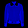
\includegraphics[width=0.3\linewidth]{chapter3/Linear/origin.png}}
    ~
    \subcaptionbox
        {RM-CI-Color-2
        \label{fig:linear-RM-CI-color-2}}
        {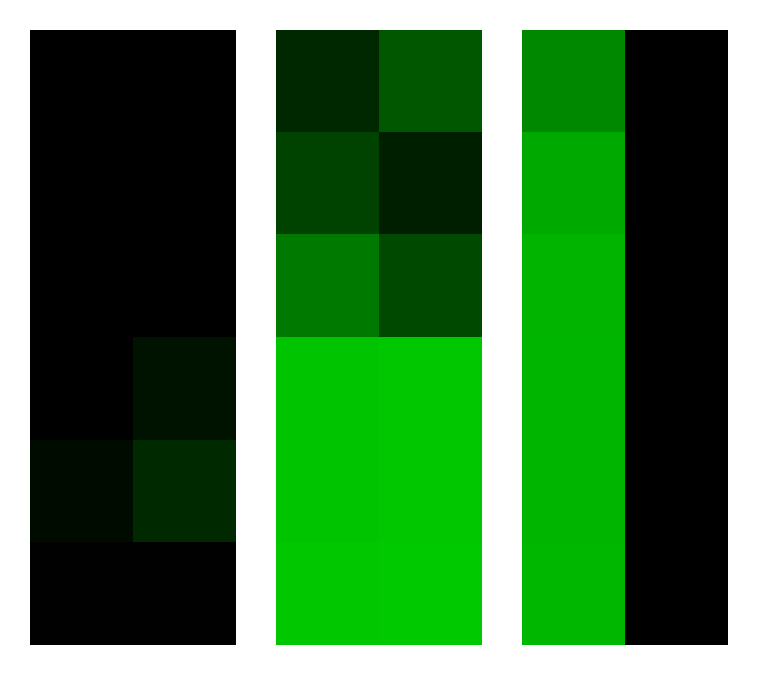
\includegraphics[width=0.3\linewidth]{chapter3/Linear/RGB_convs_2_RM_CI.png}}
    ~
    \subcaptionbox
        {RM-CI-Gray-2
        \label{fig:linear-RM-CI-gray-2}}
        {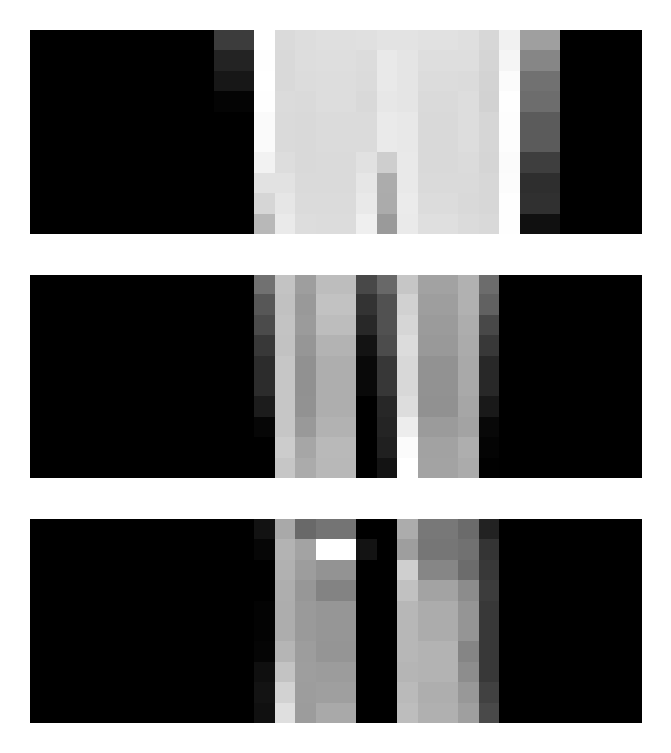
\includegraphics[width=0.3\linewidth]{chapter3/Linear/Gray_convs_2_RM_CI.png}}
    \caption{輸入影像與色彩特徵傳遞區塊和輪廓特徵傳遞區塊最後一層的RM-CI\cite{YangCNNInterpretable}}
    \label{fig:RM-CI}
\end{figure}

\begin{figure}[H]
    \centering
    \subcaptionbox
        {x * w 最大位置色彩CI
        \label{fig:linear-rgb}}
        {
\includegraphics[width=0.33\linewidth]{chapter3/Linear/Linear_color.png}}
    ~
    \subcaptionbox
        {x * w 最大位置輪廓CI
        \label{fig:linear-gray}}
        {
\includegraphics[width=0.33\linewidth]{chapter3/Linear/Linear_gray.png}}
    \caption{輸入影像與色彩特徵傳遞區塊和輪廓特徵傳遞區塊最後一層的RM-CI\cite{YangCNNInterpretable}}
    \label{fig:Linear-w-x}
\end{figure}

\end{document}